\chapter{Le Blockchain}
L'obiettivo principale delle Blockchain è quello di trasferire un bene tra due nodi di una rete in maniera affidabile e sicura. Si possono tuttavia verificare delle condizioni di fallimento, elencate di seguito:
\begin{itemize}
    \item \textbf{Modelli di fallimento}:
    \begin{itemize}
        \item \textbf{Fallimenti dei nodi} - crash o hang
        \item \textbf{Fallimenti dei link} - crash persistente o intermittente
        \item \textbf{Malfunzionamenti di rete} - perdita, alterazione o ritardo anormale di pacchetti o partizionamento della rete
    \end{itemize}
    \item \textbf{Modelli di attacco}:
    \begin{itemize}
        \item \textbf{Replay attack} - una transazione valida viene maliziosamente ripetuta o ritardata
        \item \textbf{Man-in-the-middle attack} - la comunicazione è osservata e alterata da una terza parte non autorizzata
        \item \textbf{Masquerade attack} - un nodo malizioso utilizza un'identità forgiata ad hoc per la comunicazione, oppure un nodo impersona un altro
        \item \textbf{Comportamento bizantino} - un nodo si comporta in modo non previsto
    \end{itemize}
\end{itemize}
La modalità comunemente adottata nelle transizioni finanziarie è con un mediatore, che di solito è la banca. Questa è garante in caso di manomissioni o fallimenti. Questa soluzione è implementata con il \textbf{2-phase-commit}, algoritmo distribuito per le transazioni che avvengono in database non uniformi ma splittati in più sorgenti. Il 2-phase-commit fa sì che il richiedente non contatti tutte le sorgenti del db ma che sottometta la transazione ad un mediatore che si occupa di dividerla in sottotransazioni che vengono poi inviate alle varie sorgenti del db. 

La soluzione con mediatore consente di gestire gli attacchi di tipo masquerade o bizantini, in quanto il mediatore conosce le identità delle sorgenti autorizzate, quindi può implementare meccanismi di verifica dell'identità; inoltre conosce il comportamento giusto, e può estromettere dal sistema qualsiasi nodo non rispetti quel comportamento.

\vspace{5mm}
Per inviare un bene senza la collaborazione di un'entità di terze parti si può definire un protocollo per eseguire transazioni affidabili e sicure in un ambiente inaffidabile e insicuro. L'idea è quindi di decentralizzare il sistema, ma c'è bisogno di tenere sotto controllo tre importanti proprietà: integrità del messaggio tramite hash, identità dei nodi tramite firma digitale e consenso per la validità delle transazioni.

Le valute correnti posseggono un modello di trust che si basa sul mercato e sui sistemi economici di uno stato, quindi legati alla banca centrale. Una valuta virtuale è legata direttamente ad una valuta, ma è espressa diversamente, ad esempio la valuta presente nei videogiochi. Una criptovaluta è un tipo di valuta slegata da una banca centrale e che ha valore solo nel mondo digitale. L'obiettivo della blockchain a supporto del bitcoin è di creare un ambiente decentralizzato in cui nessuna terza parte abbia il controllo delle transazioni e dei dati.

\vspace{5mm}

Le blockchain sono state teorizzate a supporto delle cosiddette criptovalute, ovvero una rappresentazione digitale di valore basata sulla crittografia e senza intermediazione. Una \textbf{criptovaluta} è una moneta creata da una soluzione computazionale decentralizzata e distribuita, governata dalla regola della maggioranza con transazioni tra due partecipanti, senza intermediazione. Le transazioni richiedono minuti e dipendono dalla qualità della rete, inoltre nessuna alterazione è possibile dopo il completamento di una transazione. Il valore di una criptovaluta viene regolato dalla domanda e dall'offerta del mercato, e non può essere manipolato in quanto la creazione dei nuovi Bitcoin è regolata matematicamente e non stampata su comando delle varie banche centrali sparse per il mondo. Non esiste in forma fisica, ma si genera e si scambia esclusivamente per via telematica.

La \textbf{moneta legale}, d'altra parte, è rilasciata dal governo ed è governata da una banca centrale, che ne fa da intermediario per le transazioni. Le transazioni locali ed internazionali possono richiedere giorni, e sono possibili alterazioni dopo il completamento di una transazione. Ha un valore grazie al fatto che esiste un'autorità (lo Stato) che agisce come se avesse questo valore. Se un'organizzazione abbastanza grande emette, usa e accetta qualcosa come pagamento, automaticamente quel qualcosa acquisisce valore. Ha un valore non coperto da riserve di altri materiali (es. riserve auree) e quindi è privo di valore intrinseco.

Le criptovalute rientrano nel caso delle valute virtuali ma sono diverse dalle valute digitali:
\begin{itemize}
    \item una valuta virtuale è una rappresentazione digitale di valore che non è né emessa da una banca centrale né da un'autorità pubblica, né necessariamente collegata a una valuta a corso legale, ma è accettata come mezzo di pagamento e può essere trasferita, archiviata, o scambiata elettronicamente.
    \item una valuta digitale è una rappresentazione nel virtuale di una valuta a corso legale.
    \end{itemize}

\section{Struttura della Blockchain}
La blockchain ha radici storiche. Anni fa esistevano dei registri chiamati \textit{libri mastri}, nei quali erano contenute tutte le transazioni eseguite tra i partecipanti di un sistema. Le operazioni sono indicate in ordine cronologico e sono possibili solo inserimenti in coda. Quindi si tratta di un\textit{"append-only multi-party system of records"}, ovvero un log di transazioni.

Una variante del libro mastro è il libro mastro distribuito, detto \textbf{ledger}, nel quale c'è un insieme di nodi che ha una copia del libro mastro. I record delle transazioni sono memorizzati in una copia locale del libro in maniera sequenziale sottoforma di blocchi ordinati temporalmente\footnote{Questa tecnologia viene chiamata \textit{Distribuited Ledger Technology}}. Affinché i blocchi siano considerati validi, i partecipanti devono raggiungere un consenso. Ogni blocco (ad eccezione del genesis block) contiene un'informazione (di solito l'hash) del blocco precedente nella catena.

\vspace{5mm}

Un \textbf{blocco} è una collezione di transazioni, ed è una struttura dati divisa in tre parti: 
\begin{itemize}
    \item \textbf{nonce} (ctr): in genere chiamato intestazione del blocco,
    \item \textbf{dati} (x): dipende dall'applicazione: in Bitcoin memorizza i dati finanziari, in Ethereum memorizza i dati del contratto, in Namecoin memorizza i dati del nome.
    \item \textbf{riferimento} (s): contiene il riferimento al blocco precedente.
\end{itemize}
Il sistema garantisce che i blocchi siano sempre validi. Se un blocco viene modificato, l'hash contenuto nel blocco successivo non è più valido. L'immutabilità garantisce di evitare modifiche a qualsiasi transazione sia stata già validata.

\subsection{Funzioni Hash}
Le funzioni di hash restituiscono una stringa di poche centinaia di bit - e comunque di lunghezza fissata - (definita hash o impronta digitale) a partire da una sequenza di bit di lunghezza arbitraria. La possibilità che due sequenze di bit sottomesse alla stessa funzione di hash diano origine allo stesso valore (collisione) è definita \textit{paradosso del compleanno}, rifacendosi al famoso paradosso della probabilità.

Una funzione di hash che produce un risultato su N bit sarà reputata insicura quando verranno generati $2^{\frac{N}{2}}$ risultati in quanto si ha la probabilità di oltre il 50\% di aver trovato una collisione. Il risultato evidentemente è ben al di sotto dei $2^{N-1}$ elementi necessari suggeriti dall'intuito.

Le funzioni di hash crittografiche cercano di rendere computazionalmente inammissibile trovare due sequenze che producono la stessa impronta.

\vspace{5mm}

Nella Blockchain, un blocco è collegato al precedente mediante un hash del blocco precedente. La modifica di un blocco della catena da parte di un nodo comporterebbe la generazione di un valore di hash differente: gli altri nodi possono verificare l'integrità dei blocchi e rifiutare modifiche di transazioni già validate. Il contesto del libro mastro è reso così immutabile.

Consideriamo un esempio nel quale un utente desidera archiviare un file su un server; il file ha un nome F e un contenuto D; gli utenti desiderano recuperare il file F in un secondo momento. Vediamo cosa accade nel dettaglio:
\begin{itemize}
    \item l'utente invia il file F con il contenuto D al server;
    \item il server archivia (F,D);
    \item l'utente elimina D;
    \item l'utente richiede F dal server;
    \item il server restituisce D;
    \item l'utente ha recuperato D.
\end{itemize}
Ma cosa succede se il server è contraddittorio e restituisce D' $\neq$ D? Banalmente, l'utente potrebbe non eliminare D e quando il server restituisce D'. l'utente confronta D e D'. Ma cosa succede se l'utente non dispone di memoria sufficiente per archiviare D per molto tempo? Può usare le funzioni hash:
\begin{itemize}
    \item l'utente invia il file F con i dati D al server;
    \item il server archivia (F,D);
    \item l'utente memorizza H(D) ed elimina D;
    \item l'utente richiede F dal server;
    \item il server restituisce D';
    \item l'utente confronta H(D') = H(D).
\end{itemize}
Tuttavia ci sono soluzioni migliori: i file infatti vengono divisi in chunk, e viene calcolato l'hash di ogni chunk utilizzando una funzione hash crittografica (SHA256). Dopodiché gli hash vengono combinati a due a due costruendo quello che viene chiamato \textbf{albero di Merkle}\footnote{Vedi par. 1.2.5.}.

Gli alberi di Merkle vengono ampiamente utilizzati nella Blockchain per controllare le \textit{proof of inclusion} di una transazione all'interno del blocco dati.

\subsection{Funzioni di sicurezza}
Sebbene applicate a problemi in cui si vuole fare a meno di \textit{trusted entities}, le tecnologie blockchain utilizzano anch'esse la firma digitale (e le \textit{trusted authorities} di certificazione) per problemi di sicurezza tipici dei sistemi distribuiti:
\begin{itemize}
    \item \textbf{Authentication}: autenticazione dei nodi della rete;
    \item \textbf{Integrity}: verifica di violazioni dell'integrità dei messaggi scambiati;
    \item \textbf{Non-repudiation}: non ripudio da parte dei nodi dei messaggi inviati.
\end{itemize}
Si consideri un nodo che desidera "vendere" un bene attraverso una transazione. Il nodo predispone da sé la transazione, che deve sottoporre agli altri nodi affinché sia validata da una maggioranza. È possibile che il nodo provi a "spendere" concorrentemente due volte lo stesso bene (double spending): ciò può avvenire in maniera consapevole (comportamento bizantino) o in maniera inconsapevole (malfunzionamenti di rete, replay attack). La validità di transazione è un problema di consenso.

\vspace{5mm}

Un primo passo per risolvere il problema del \textit{double spending} è determinare se un messaggio è "fresco" o è una copia ritrasmessa. È necessario poter identificare univocamente un messaggio contenente un blocco di transazioni eseguite. Un \textbf{nonce} è definito come \textit{"a time-varying value that has at most a negligible chance of repeating, e.g., a random value that is generated anew for each use, a timestamp, a sequence number, or some combination of these."} [NIST SP-800-90]. Un nonce quindi può essere ottenuto attraverso un timestamp. Per garantire che ogni blocco sia caratterizzato da un valore differente è necessario che tale valore sia generato da una fonte fidata. L'ideale sarebbe effettuare un ordinamento totale su tempo locale, ma come sappiamo non è fattibile a causa della natura distribuita del sistema.

\section{Il tempo nei sistemi distribuiti}
In un sistema distribuito, ogni nodo è dotato di un proprio orologio, ed è possibile che ad un evento x, che accade "dopo" un altro evento y, sia associato un istante "antecedente" quello di y: ciò comporta problemi in molte applicazioni.
L'occorrenza di una singola azione in p\textsubscript{i} è un evento e. L'insieme degli eventi di un processo p\textsubscript{i} può essere ordinato totalmente in base alla relazione di \textbf{precedenza temporale}:

\vspace{5mm}

\begin{center}
    $e \rightarrow e'$ se e solo se $e$ si è verificato prima di $e'$ in p\textsubscript{i}.
\end{center}

\vspace{5mm}

L'ordinamento è ben definito (anche in caso di multithreading) in quanto ciascun processo è in esecuzione su un processore dedicato. La storia (history) di un processo p\textsubscript{i} è la successione di eventi che ha luogo in p\textsubscript{i}, ordinata in base alla relazione $\rightarrow$:

\vspace{5mm}

\begin{center}
    storia(p\textsubscript{i}) = h\textsubscript{i} = <$e_{i}^{0}, e_{i}^{1}, e_{i}^{2}, ...$>
\end{center}

\vspace{5mm}

Per marcare gli eventi viene utilizzato un orologio fisico. 

\subsection{Orologi fisici}
Un orologio fisico di un computer (computer clock, meglio detto \textit{timer}), è un dispositivo tipicamente costituito da:
\begin{itemize}
    \item un cristallo di quarzo, che oscilla a una frequenza nota;
    \item un registro contatore;
    \item un registro di inizializzazione;
    \item un registro di memorizzazione.
\end{itemize}
Ciascuna oscillazione del cristallo decrementa il contatore di una unità. Quando il contatore raggiunge lo zero, viene reimpostato al valore indicato dal registro di inizializzazione.

Il clock può dunque essere programmato per generare interruzioni periodiche (clock tick) ad esempio 60 volte al secondo. Ad ogni interruzione, il valore del registro di memorizzazione viene aggiornato. Il risultato è il valore di un clock hardware H\textsubscript{i}(t). 

Il sistema operativo legge dal registro il valore H\textsubscript{i}(t) del clock hardware, lo moltiplica per un fattore di scale ed aggiunge un offset, fornendo il valore di un clock software: C\textsubscript{i}(t) = $\alpha$ H\textsubscript{i}(t) + $\beta$. Il clock software rappresenta una misura approssimata del tempo effettivo $t$ per il processo p\textsubscript{i}.

A due eventi successivi possono essere associati valori distinti di C\textsubscript{i}(t) solo se la risoluzione del clock (periodo tra gli aggiornamenti del clock) è minore dell'intervallo temporale tra i due eventi.

\vspace{5mm}

Il \textbf{tempo effettivo} (o reale) $t$ è il tempo "vero" in ciascun istante, in un sistema di riferimento assoluto nominale, indicato da un ideale orologio di riferimento perfetto. Distinguiamo poi altri attributi:
\begin{itemize}
    \item \textbf{Clock offset}: differenza tra la lettura istantanea del clock locale rispetto a $t$ (o rispetto a un altro clock);
    \item \textbf{Clock frequency}: il tasso con cui il clock locale progredisce (derivata prima rispetto a $t$);
    \item \textbf{Clock skew}: differenza tra le frequenze del clock locale e reale;
    \item \textbf{Clock drift}: variazione nel tempo della frequenza del clock locale (derivata seconda del clock locale rispetto a $t$);
    \item \textbf{Clock adjustment}: variazione subitanea degli attributi di un clock locale, per effetto di un'azione di sistema o di utente.
\end{itemize}
Spesso la differenza tra le letture di due orologi viene indicata con il termine \textit{clock skew}, anziché \textit{clock offset}. Nei sistemi basati su blockchain i timestamp devono essere più vicini possibili a meno di un errore minimale.

\subsection{Sincronizzazione dei clock}
Per molte applicazioni l'ora "effettiva" è fondamentale, per cui sono spesso necessari orologi fisici esterni. Per ragioni di efficienza e affidabilità gli orologi sono tipicamente ridondanti. Si pongono due tipi di problemi:
\begin{itemize}
    \item \textbf{sincronizzazione esterna}: ovvero come sincronizzare un orologio locale con un orologio esterno - algoritmo di Cristian (1989);
    \item \textbf{sincronizzazione interna}: ovvero come sincronizzare più orologi tra loro - algoritmo di Berkeley (1989).
\end{itemize}

\subsection{Algoritmo di Cristian}
È un algoritmo di sincronizzazione esterna che si basa sull'utilizzo di un time server passivo, dotato di un dispositivo che riceve il segnale di una sorgente UTC. Su richiesta, un processo server invia un messaggio contenente l'ora $t$, misurata col proprio orologio basato su UTC.

\begin{figure}[ht]
    \centering
    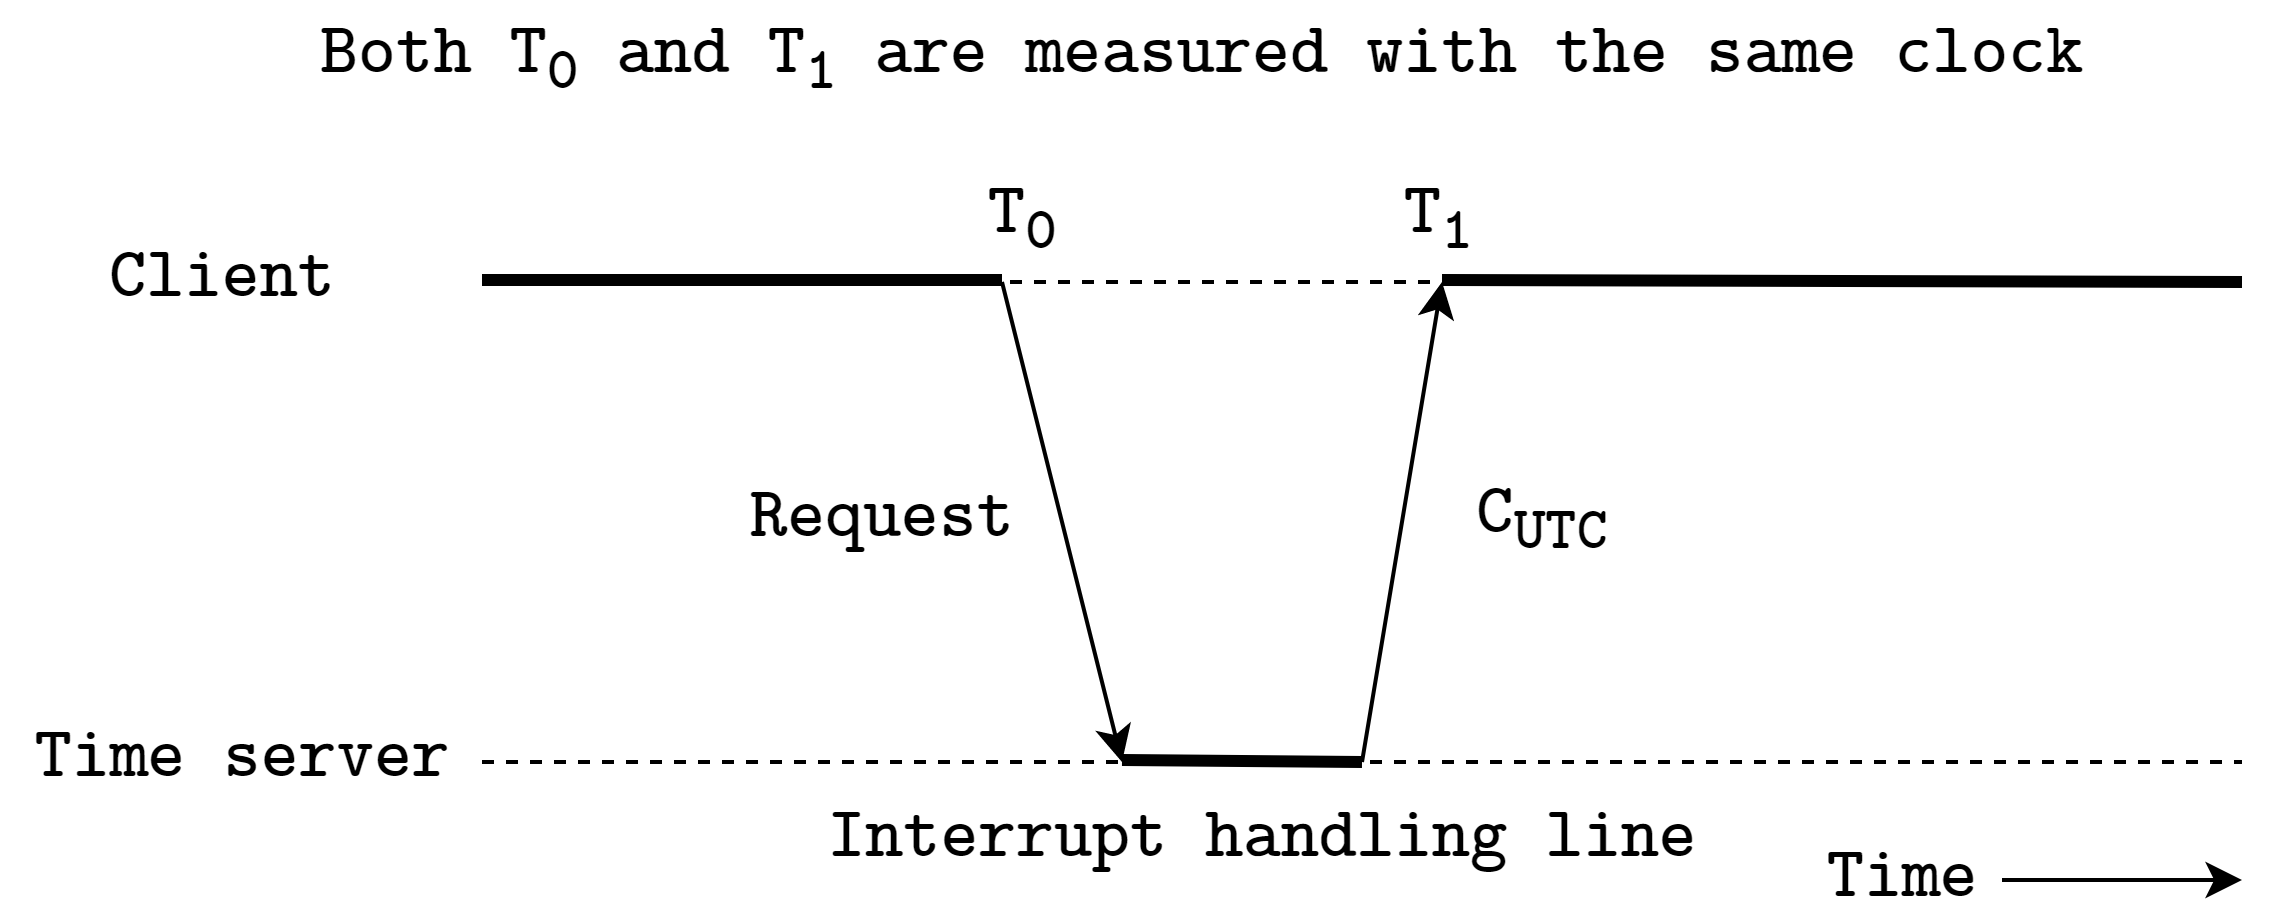
\includegraphics[width=8cm]{./Images/cap3/3.1.png}
\end{figure}

Il processo cliente $p$ misura il \textit{round trip time} $T_{RTT}$ come intervallo temporale tra gli istanti $T_{0}$ e $T_{1}$. L'accuratezza della misura dipende dal clock drift. Tipicamente si può assumere che $p$ possa poi aggiornare il clock locale al valore $(t + T_{RTT})/2$.

\vspace{5mm}

Cristian definisce il suo algoritmo probabilistico: si raggiunge la sincronizzazione solo se il \textit{round trip time}(RTT) dei messaggi è sufficientemente piccolo rispetto all'accuratezza richiesta. Ad esempio, su una rete LAN, il RTT generalmente non supera i 10 ms. Un clock con un drift rate di $10^{-6}$ secondi al secondo varia non più di $10^{-5}$ ms.

Detto \textit{min} il tempo minimo di trasmissione dei messaggi, l'ora dell'orologio del server all'istante $T_{1}$ è compresa in [$t + min, t + T_{RTT} min$], con intervallo ampio $2 T_{RTT} min$. L'accuratezza è quindi $\pm (T_{RTT}/2 min)$.

\subsection{Algoritmo di Berkeley}
È un algoritmo di sincronizzazione interna ideato principalmente per reti intranet. Si basa sull'utilizzo di un time server attivo: un nodo viene selezionato come \textbf{master}, gli altri nodi con cui deve essere effettuata la sincronizzazione fanno da \textbf{slave}.

Il master deve:
\begin{itemize}
    \item effettuare periodicamente il polling dei nodi slave;
    \item calcolare una stima dell'ora locale di ciascuno slave, in base al \textit{round trip time} (come nell'algoritmo di Cristian);
    \item calcolare l'ora media (inclusa la propria);
    \item comunicare ad ogni slave di quanto variare il clock locale.
\end{itemize}
L'accuratezza dell'algoritmo dipende dal round trip time dei messaggi tra il master e gli slave. Per aumentarla, il master deve:
\begin{itemize}
    \item stimare un round trip time massimo nominale;
    \item eliminare dal calcolo della media le letture dei clock associate a valori del round trip time maggiori del massimo.
\end{itemize}
In questo modo di limita l'effetto dei clock con i quali il RTT è troppo variabile.

Per aumentare ulteriormente la precisione, l'algoritmo prevede di non considerare le letture di eventuali faulty clocks. A tale scopo, il master considera nel calcolo della media solo il sottoinsieme dei clock locali che non differiscono tra essi più di un valore prestabilito. Si dice che il master effettua una media tollerante ai guasti (fault tolerant average). Nel caso in cui il master si guasti, è prevista l'elezione di un nuovo master.

\subsection{Network Time Protocol}
È un protocollo per un \textit{time service} per nodi di rete internet. L'obiettivo di NTP è di offrire ai nodi internet un servizio di sincronizzazione con l'ora UTC. Questo servizio deve essere offerto in modo:
\begin{itemize}
    \item affidabile, anche in caso di lunghe perdite di connettività;
    \item scalabile, adatto all'elevato numero di client e server su internet;
    \item sicuro, mediante meccanismi di protezione da interferenze accidentali o maliziose con il time service.
\end{itemize}
Il servizio NTP è fornito da una rete di server connessi a internet, secondo un'organizzazione logica gerarchica. 

I server NTP sono classificati in \textbf{server primari}, direttamente connessi a una sorgente UTC, e \textbf{server secondari}, sincronizzati direttamente con server primari; inoltre possono sincronizzarsi secondo tre modalità: multicast, procedure call e symmetric.
\begin{itemize}
    \item Il \textit{multicast mode} è previsto per reti LAN. Il server effettua periodicamente il multicast dell'ora ai nodi sull LAN. I nodi regolano la propria ora su quella del server.
    \item Il \textit{procedure call mode} è analogo all'algoritmo di Cristian: il server accetta richieste e risponde con la lettura corrente del proprio clock. Questa modalità è usata ad esempio dai file server su una LAN o su LAN adiacenti.
    \item Il \textit{symmetric mode} è usato dai livelli più bassi della gerarchia per raggiungere maggiore precisione.
\end{itemize}
Tutte le modalità usano messaggi UDP. In \textit{procedure call mode} e \textit{symmetric mode}, i server si scambiano coppie di messaggi che contengono l'ora locale dei due eventi-messaggio più recenti, oltre a quello corrente.

\begin{figure}[ht]
    \centering
    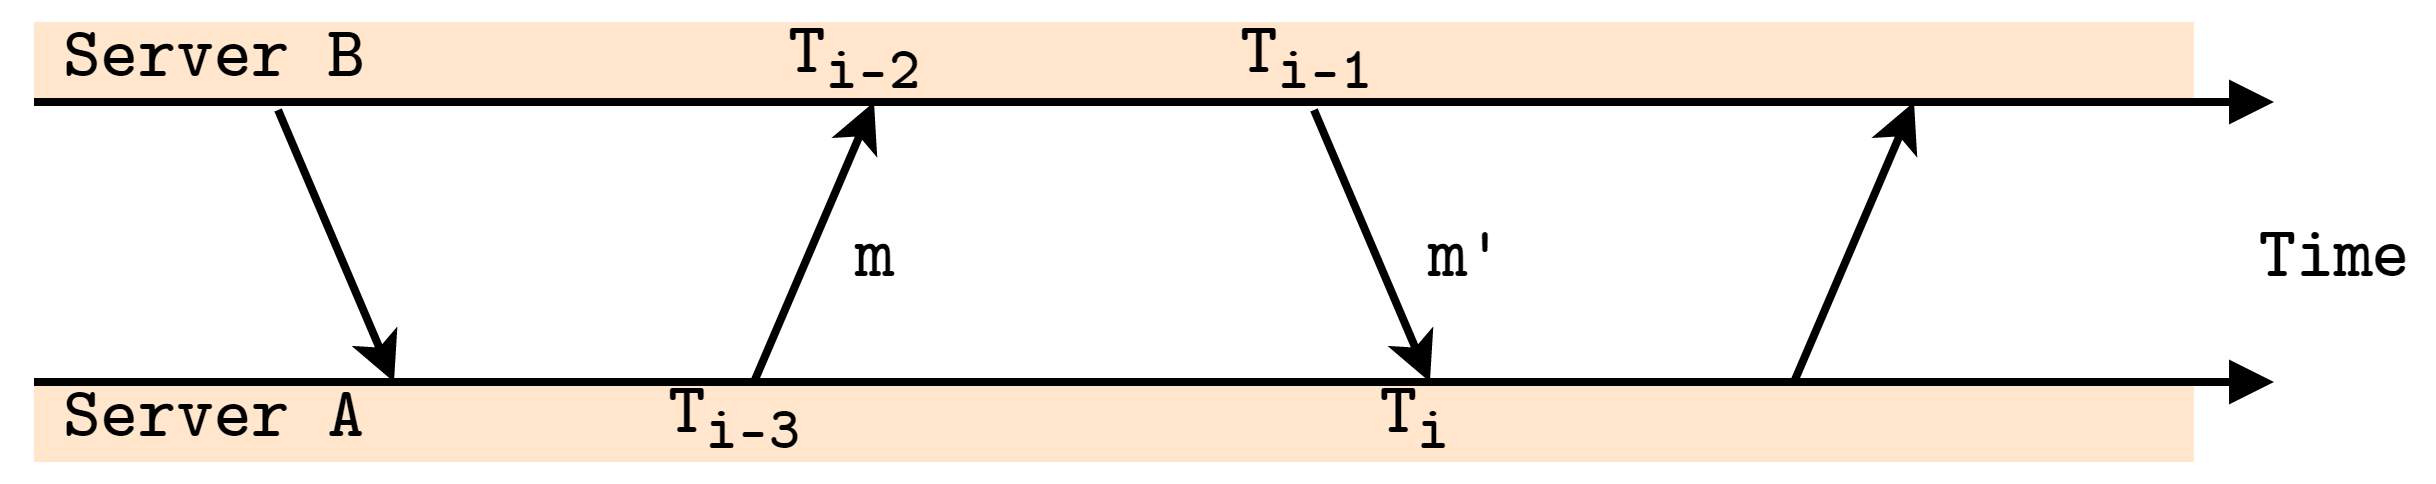
\includegraphics[width=8cm]{./Images/cap3/3.2.png}
\end{figure}

\begin{itemize}
    \item $o$: offset vero del clock di B rispetto a quello di A
    \item $t, t'$: tempi di trasmissione effettivi di $m, m'$
    \item $T_{i-2} = T_{i-3} + t + o$
    \item $T_{i} = T_{i-1} + t' - o$
\end{itemize}
Per ogni coppia di messaggi vengono calcolati:
\begin{itemize}
    \item il delay $d_{i} = t + t' = T_{i-2} - T_{i-3} + T_{i} - T_{i-1}$
    \item una stima dell'offset $o_{i} = (T_{i-2} - T_{i-3} + T_{i-1} - T_{i})/2$
\end{itemize}
Si ha che:
\[ o = o_{i} + (t' - t)/2 \quad o_{i} - d_{i}/2 \leq o \leq o_{i} + d_{i}/2\]
L'accuratezza della stima $o_{i}$ è misurata da $d_{i}$.

\vspace{5mm}

La relazione tra eventi \textbf{Happened- before} (HB), indicata con il simbolo $\rightarrow$, è definita dalle condizioni:
\begin{itemize}
    \item HB1: se esiste un processo $ p_{i}$ tale che $e \rightarrow_{i} e'$ (cioè $p_{i}$ osserva che $e$ accade prima di $e'$), allora $e \rightarrow e'$
    \item HB2: per ogni messaggio $m$, \texttt{send(m)} $\rightarrow$ \texttt{receive(m)}
    \item HB3: se $e \rightarrow e'$ e $e' \rightarrow e''$, allora $e \rightarrow e''$ (proprietà transitiva)
\end{itemize}
La relazione \textit{happened-before} definisce un ordinamento parziale degli eventi in un sistema distribuito. Nel grafico seguente è mostrato un esempio.

\begin{figure}[hbt!]
    \centering
    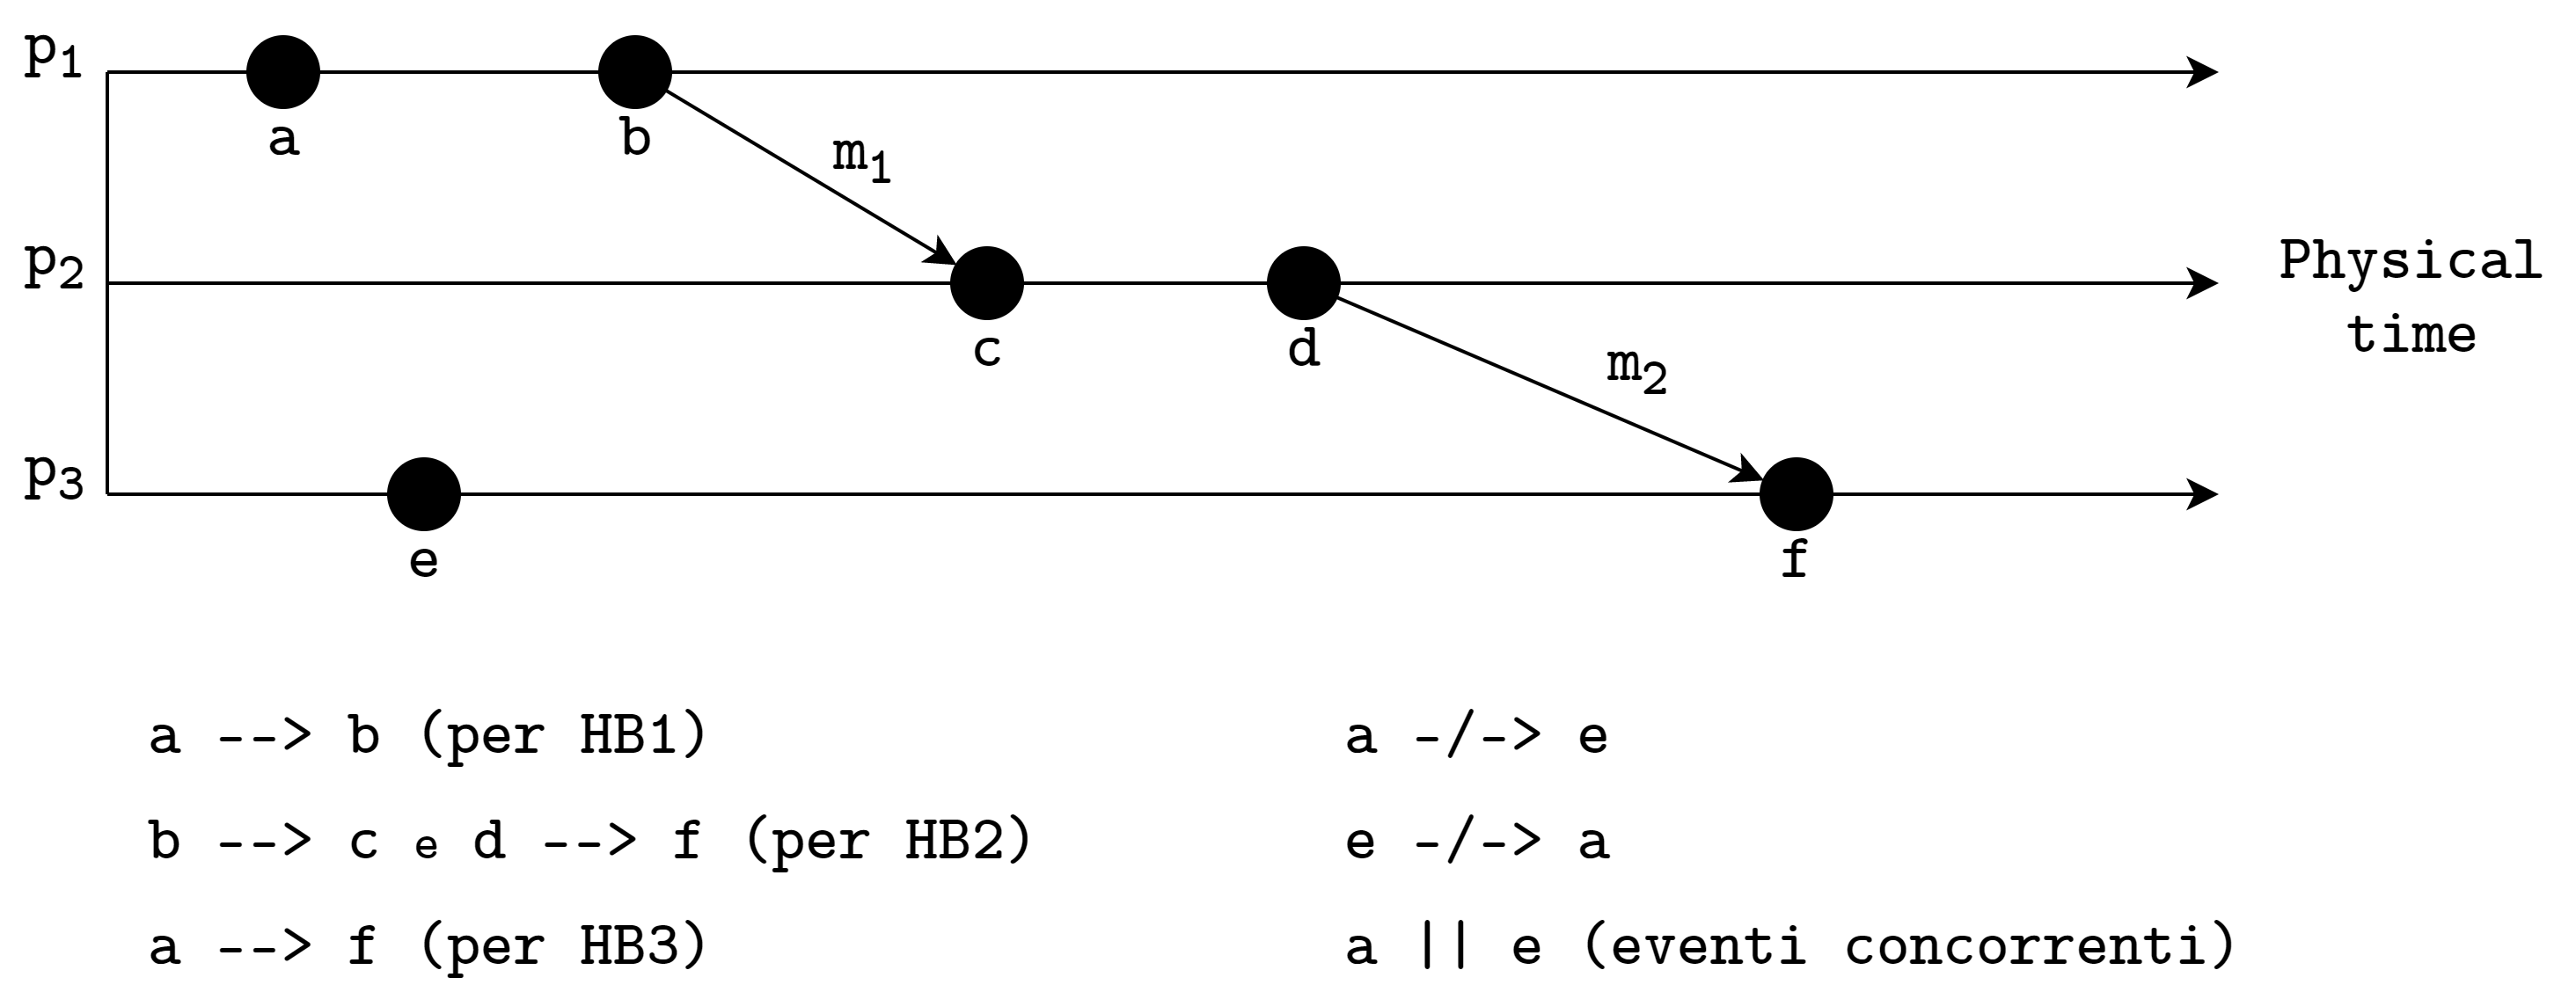
\includegraphics[width=10cm]{./Images/cap3/3.3.png}
\end{figure}

\subsection{Orologi logici}
Lamport ha ideato un semplice meccanismo (logical clocks) con cui esprimere numericamente la relazione HB tra eventi in un sistema distribuito.

Un orologio logico di Lamport (LC, o LLC) è un contatore software crescente monotonicamente; i suoi valori (interi) non sono necessariamente in relazione con quelli di un orologio fisico. Un LC viene tipicamente incrementato di 1, ma si può scegliere qualsiasi valore intero. 

Ogni processo ha il suo LC, che usa per marcare temporalmente gli eventi: $L_{i}(e)$ è la marcatura di $e$ da parte del processo $p_{i}$ che lo osserva (Lamport timestamp). Ogni processo aggiorna il proprio LC e lo invia insieme ai messaggi che trasmette, in base alle seguenti regole:
\begin{itemize}
    \item LC1: $L{i}$ è incrementato prima di ogni evento osservato da $p_{i}$
    \begin{itemize}
        \item $L_{i} := L_{i} + 1$
    \end{itemize}
    \item Quando $p_{i}$ invia un messaggio $m$, inserisce in $m$ il valore $t = L_{i}$ e chiama \texttt{send(m)}
    
    \item Quando $p_{j}$ riceve $(m,t)$ calcola $L_{j} := max(L_{j},t)$ e applica LC1 prima di marcare l'evento \texttt{receive(m)}
\end{itemize}

\begin{figure}[hbt!]
    \centering
    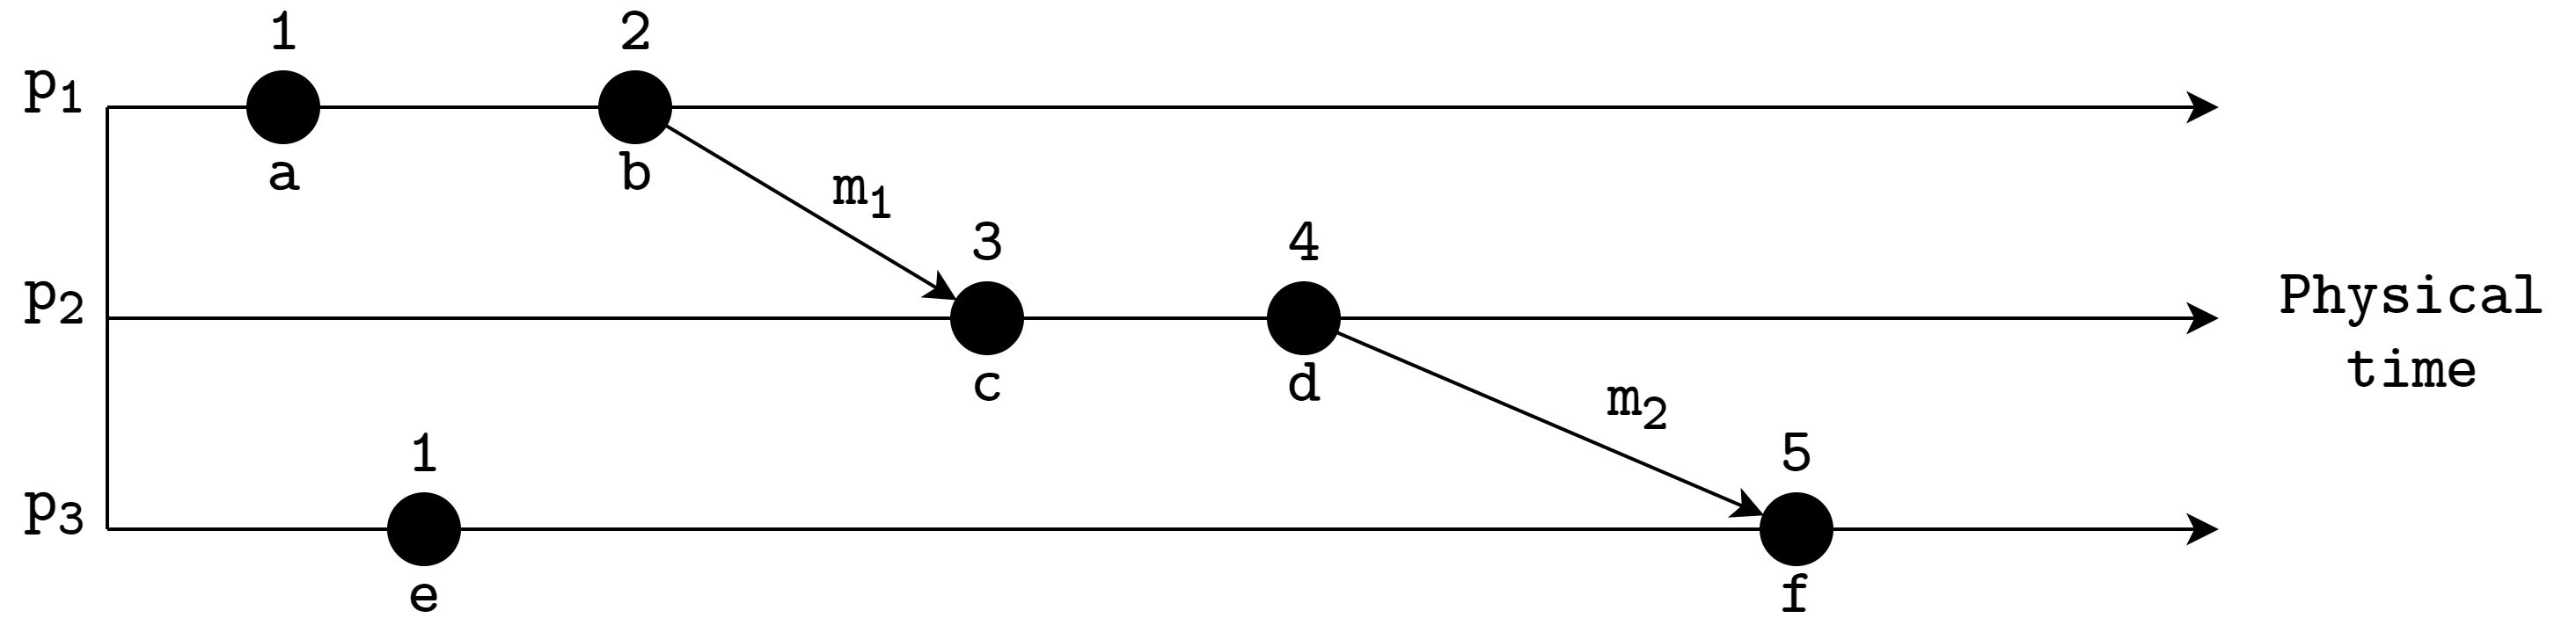
\includegraphics[width=10cm]{./Images/cap3/3.4.png}
\end{figure}

Banalmente, per induzione vale che:

\[ e \rightarrow e' \Rightarrow L(e) < L(e')\]

Non vale il contrario, quindi non possiamo infierire l'ordine relativo di due eventi conoscendo le loro marche temporale. Infatti nell'immagine precedente vale che $L(b) > L(e)$ ma $b || e$.

Negli orologi logici è possibile manomettere le marcature temporali in quanto si basano sul corretto scambio di messaggi.

\subsection{Orologi vettori}
Un orologio vettore (VC) per un sistema di N processi è un array di N interi. Ogni processo detiene un proprio orologio vettore $V_{i}$ e aggiorna il proprio VC, inviandolo assieme ai messaggi che trasmette, in base alle seguenti regole:
\begin{itemize}
    \item VC1: inizialmente, $V_{i}[j] = 0$ con $i, j = 1, 2, ..., N$
    \item VC2: $V_{i}[i]$ è incrementato prima di ogni evento osservato da $p_{i}: V_{i}[i] := V_{i}[i] + 1$
    \item VC3: quando $p_{i}$ invia un messaggio $m$, inserisce in $m$ il vettore $t = V_{i}$
    \item VC4; quando $p_{i}$ riceve $(m,t)$, calcola $V_{i}[j] := max(V_{i}[j],t[j])$ con $j = 1, 2, ..., N$
\end{itemize}
Il valore in $V_{i}[i]$ rappresenta il numero di eventi che $p_{i}$ ha marcato. Il valore in  $V_{i}[j]$ ($i \neq j$) rappresenta il numero di eventi osservati da $p_{j}$ e dai quali $p_{i}$ è causalmente potenzialmente affetto ($p_{j}$ potrebbe aver marcato più eventi, ma di questi non è pervenuta informazione a $p_{i}$).

\begin{figure}[hbt!]
    \centering
    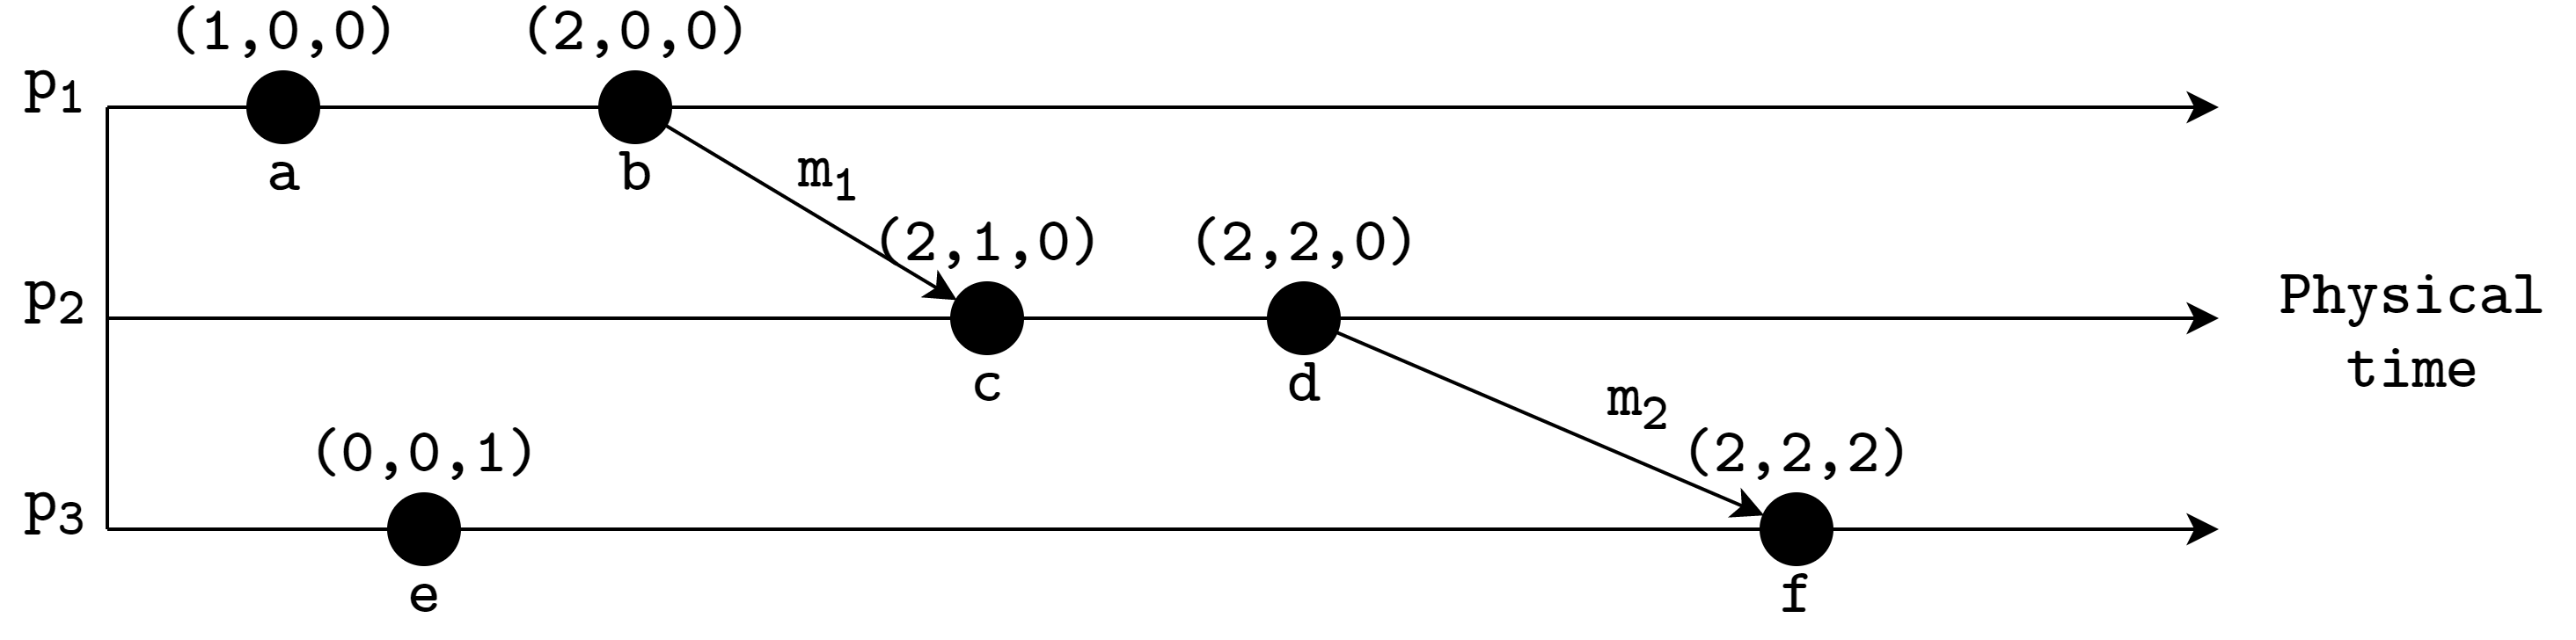
\includegraphics[width=10cm]{./Images/cap3/3.5.png}
\end{figure}

Rispetto agli orologi scalari di Lamport, gli orologi vettore richiedono una occupazione di memoria e un \textit{payload} nei messaggi proporzionale al numero di processi N.

È lecito chiedersi se questo costo - oltre che sufficiente - sia necessario per poter stabilire quale tra due eventi sia in relazione HB con l'altro ispezionando solamente le marcature temporali.

In effetti, è stato dimostrato (Charron-Bost, 1991) che se si vuole stabilire l'ordinamento relativo tra due eventi in base ad orologi logici, un costo proporzionale a N è inevitabile. Naturalmente, se N è molto grande è possibile adoperare opportune tecniche di compressione per ridurre l'occupazione di memoria e il payload dei messaggi.

\subsection{Certificazione del tempo}
La certificazione del tempo serve a verificare quando un documento è stato creato, oppure quando è stata apportata l'ultima modifica in maniera affidabile e non falsificabile. Si impiega un \textit{Trusted Time Server} (TTS).
\begin{itemize}
    \item Prima soluzione: l'utente invia al TTS una copia del documento, e il TTS aggiunge data e ora e conserva il documento nella cassetta di deposito.
    \item Seconda soluzione: si impiega una primitiva crittografica per proteggere la privacy del documento, e ridurre i costi di trasmissione e memorizzazione: l'utente invia al TTS l'hash del documento. Il TTS aggiunge data, ora e firma e invia questo certificato all'utente.
\end{itemize}
Indipendentemente dalla correttezza del tempo certificato, si vuole che due documenti sottoposti sequenzialmente al TTS abbiano un nonce che esprima questa sequenzialità. Ogni certificato rilasciato contiene l'hash del documento, data, ora, firma del TTS e l'hash del certificato precedente o parte di esso. Complessivamente i certificati formano una catena di blocchi. È inammissibile inserire successivamente un certificato all'interno della catena, il TTS dovrebbe rilevare collisioni per la funzione hash.

Questa soluzione comporta una serie di vantaggi:
\begin{itemize}
    \item aggiungere il timestamp rende l'hash più resistente rispetto alle collisioni;
    \item risolve il problema del \textit{double spending} assegnando un ordine temporale alle transazioni e pubblicandole.
\end{itemize}
Per svincolarsi dall'utilizzo di un timestamp server, alcune soluzioni blockchain sfruttano un meccanismo differente per la generazione dei nonce. Tale meccanismo è definito \textbf{Proof-of-Work} (PoW). Per proporre un nuovo blocco da aggiungere al \textbf{ledger}, un nodo deve dimostrare di aver utilizzato abbastanza risorse di calcolo per risolvere un enigma matematico, il cui risultato è inserito nel blocco stesso. La PoW implica la computazione di un valore di hash con un determinato numero di bit iniziali pari a zero. Ogni nodo (detto \textit{miner}) cerca di trovare un nonce tale da soddisfare il vincolo sul numero di zero prodotti dalla funzione di hash.

Il lavoro medio richiesto è esponenziale rispetto al numero di bit zero richiesti e può essere verificato eseguendo un singolo hash. Tale operazione è molto onerosa dal punto di vista computazionale e richiede la collaborazione di diverse CPU e GPU per poter essere realizzata.

\subsection{Transazioni con consenso distribuito}
Tutti i nodi della rete sono a conoscenza di tutte le transazioni e partecipano attivamente alla validazione dei blocchi attraverso il raggiungimento del consenso. Il modello di sicurezza deve contemplare anche il cosiddetto \textit{51\% attack}, nel quale un gruppo di nodi maliziosi possiede più del 50\% della potenza computazionale della rete.

Nessun algoritmo può garantire il raggiungimento del consenso in un sistema asincrono nel caso di anche un unico fallimento per crash di un processo (\textbf{Teorema di Impossibilità}). Per raggiungere il consenso in sistemi asincroni in presenza di fallimenti si possono rilassare i vincoli di consenso oppure rendere meno asincrono il sistema, sfruttando i periodi di sincronia.

\vspace{5mm}

È consentito che in alcuni casi non si raggiunga il consenso tra tutti i nodi della rete, ovvero solo un sottoinsieme di nodi raggiungono il consenso. In questo caso è possibile un 51\% attack. Esistono molte soluzioni diverse che consentono di irrobustire il consenso per evitare questo tipo di attacchi, ad esempio l'aggiunta di un controllo collettivo, dove chiunque valida una transazione deve spendere tanto tempo computazionale in modo da scoraggiare l'attacco, oppure è previsto un meccanismo di incentivazione: una ricompensa per il lavoro svolto.

Il rilassamento dei vincoli di consenso può dare origine a biforcazioni della blockchain (\textbf{Blockchain Forking}). Nel caso di produzione simultanea di due blocchi, alcuni blocchi aggiungeranno alla propria blockchain il blocco rosso ed altri il blocco blu, fino ad arrivare alla realizzazione di una \textit{forked blockchain}, che rappresenta la situazione di non consenso.

\begin{figure}[hbt!]
    \centering
    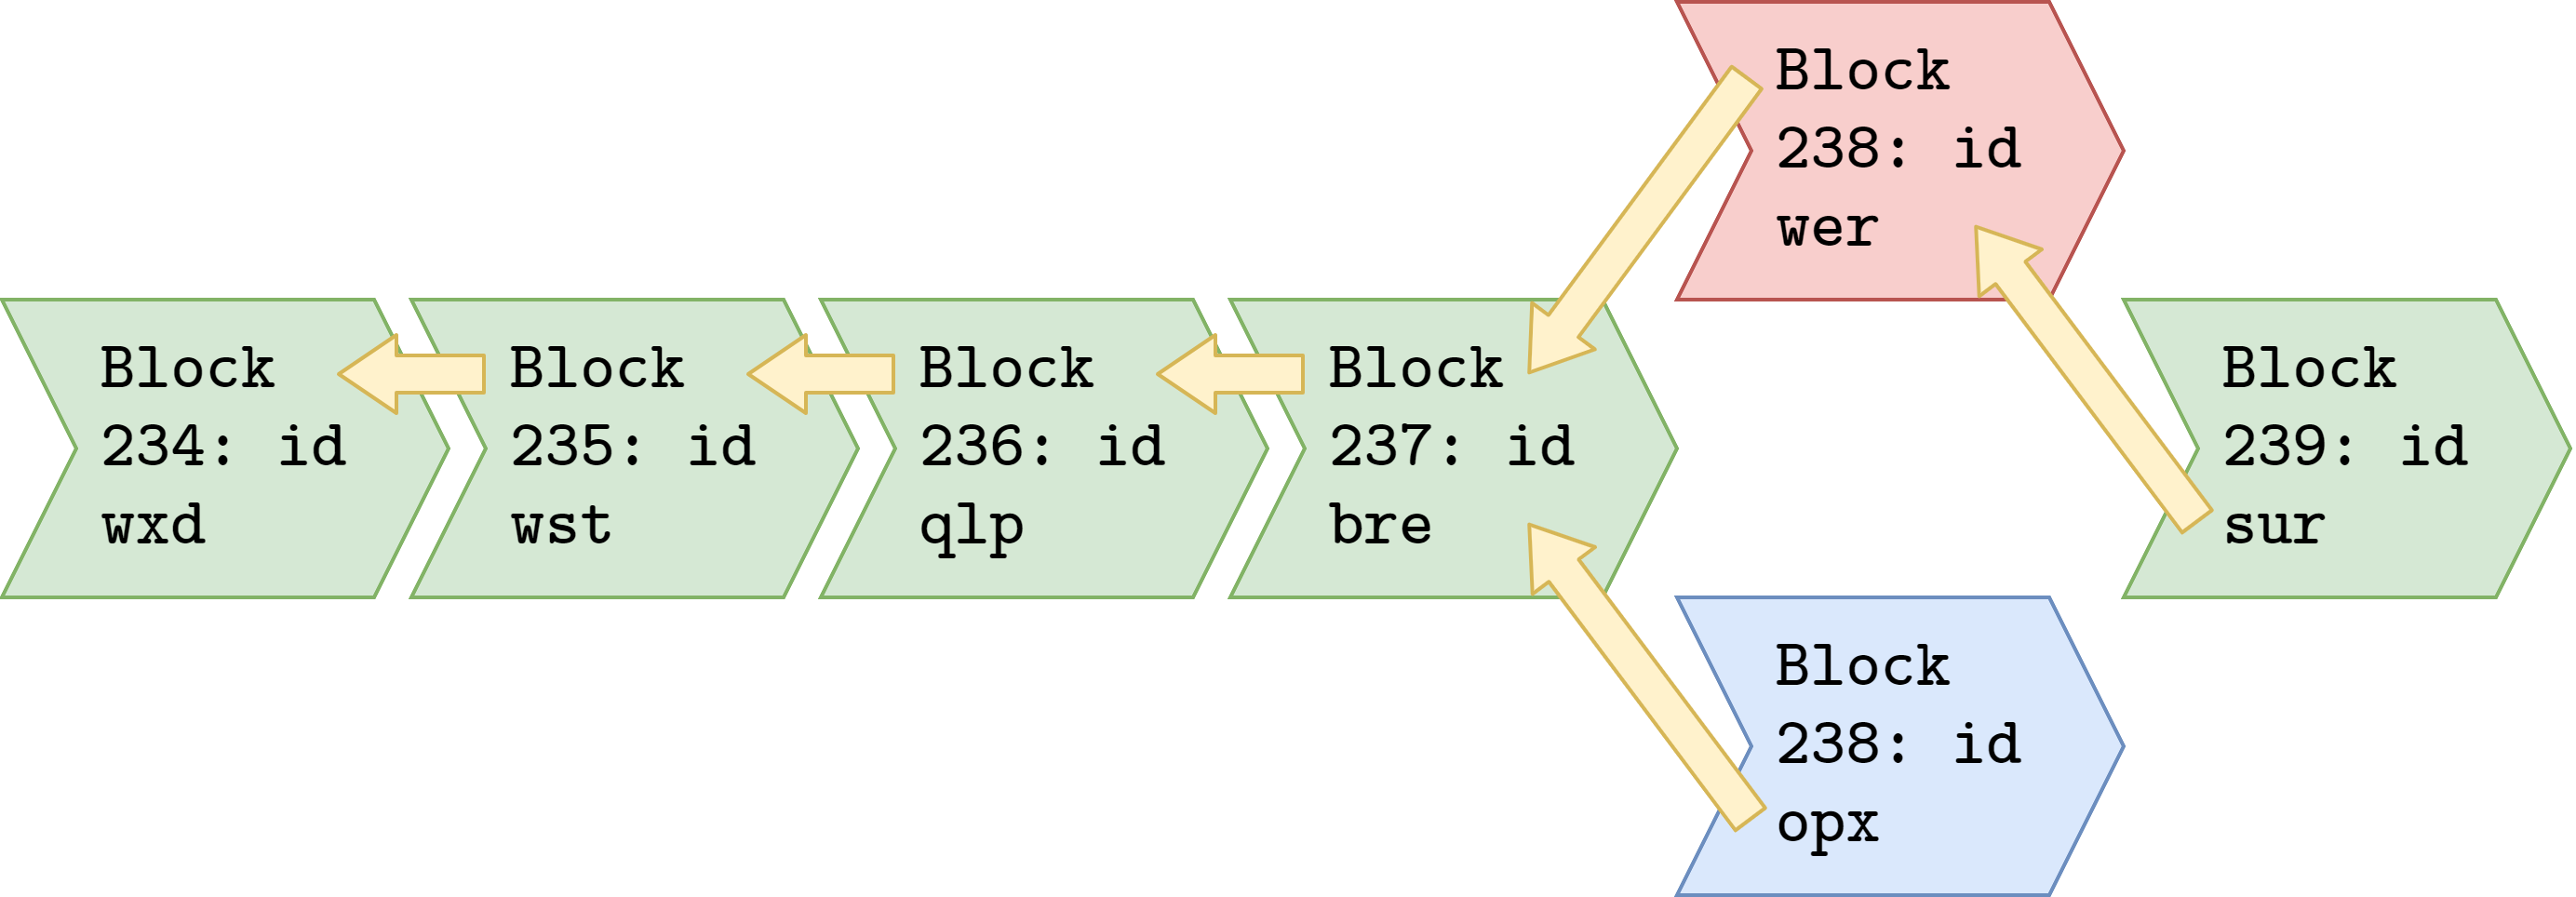
\includegraphics[width=8cm]{./Images/cap3/3.6.png}
\end{figure}

All'atto della produzione del blocco successivo, esso farà riferimento ad uno solo dei due blocchi precedentemente creati. Tale operazione comporta la rimozione del ramo della blockchain composto del nodo blu, in quanto predomina il ramo di lunghezza maggiore. Il consenso è raggiunto.

In un certo istante di tempo la comunità può ritenere necessario cambiare le regole della blockchain in modo che determinate transazioni ritenute non valide fino a quel momento siano considerate valide da tale istante e nel futuro. Tale condizione genera un \textbf{hard fork}, che comporta la generazione voluta di un nuovo ramo della blockchain per distinguere i nodi che seguono il nuovo regolamento rispetto a quelli fedeli al vecchio. In qualsiasi momento i nodi possono decidere di abbandonare un ramo per seguire l'altro.

\subsection{Consenso Nakamoto - Bitcoin}
Un metodo per ottenere il consenso è utilizzare l'algoritmo del consenso Nakamoto - Bitcoin, che funziona come segue:
\begin{enumerate}
    \item Ogni nuova transazione viene inviata in broadcast a tutti i nodi;
    \item Ogni nodo collezione le nuove transazioni in un blocco;
    \item Ogni nodo cerca un PoW difficile per il proprio blocco. La PoW consiste nel calcolo di un valore (un nonce) tale che un hash di blocco + il nonce inizi con un numero di zeri stabilito;
    \item Quanto un nodo trova una PoW, invia in broadcast a tutti i nodi il blocco contenente le transazioni e la PoW;
    \item Un nodo accetta il blocco solo se:
    \begin{itemize}
        \item tutte le transazioni sono valide;
        \item le transazioni non sono relative ad un bene già speso;
        \item la PoW è valida. A tale scopo il nodo calcola a sua volta l'hash del blocco, e verifica che abbia lo stesso numero di zeri iniziali.
    \end{itemize}
    \item I nodi manifestano l'accettazione del blocco aggiungendolo alla blockchain all'atto della creazione del blocco successivo, utilizzando l'hash del blocco accettato per creare il prossimo blocco.
\end{enumerate}
Due nodi possono fare concorrentemente il broadcast di blocchi differenti, e nodi diversi possono ricevere i due broadcast in ordine diverso. Ciascun nodo lavora sul primo blocco che riceve, ma conserva l'altro ramo. L'indecisione si risolve quando un ramo diventa più lungo: i nodi che lavorano sul ramo meno lungo lo abbandonano e proseguono a lavorare sulla catena più lunga.

È opportuno incoraggiare la cooperazione dei nodi alla creazione del consenso (validazione delle transazioni corrette): affinché un blocco sia validato ci deve essere una maggioranza di nodi corretti e che spendono risorse (costruendo la PoW). Poiché la PoW è onerosa, anche i nodi corretti potrebbero non essere ben disposti a cooperare. È prevista allora una politica di incentivi, che consiste nell'incoraggiare i processi corretti a collaborare nonostante l'onere computazionale, mettendo in minoranza i processi maliziosi. Questi ultimi dovranno avere ancora più potenza di calcolo per contrastare molti nodi corretti che validano il blocco.

La prima transazione di ogni blocco assegna un compenso al nodo creatore del blocco (ed ecco perché il data mining è molto diffuso).

\section{Definizione base di Blockchain}
Una \textbf{Blockchain} è un libro mastro pubblico distribuito (distribuited public ledger) di transazioni o eventi digitali eseguiti e condivisi tra i partecipanti. Ogni transazione riportata nella blockchain è validata tramite il raggiungimento del consenso tra i nodi del sistema. Una volta memorizzate, le informazioni non possono essere cancellate né modificate. Ogni blocco contiene uno o più record (un record per transazione), e come in un libro mastro, la storia delle registrazioni è immutabile e può essere verificata a partire dal primo blocco, chiamato \textbf{genesis block}. 

Le proprietà che una blockchain fornisce sono:
\begin{itemize}
    \item \textbf{Pubblica verificabilità}: ogni transazione può essere verificata da ogni partecipante (tramite gli alberi di Merkle)
    \item \textbf{Trasparenza}: ogni partecipante ha accesso ad un sottoinsieme di informazioni
    \item \textbf{Privacy}: l'identità di chi esegue una determinata transazione è tutelata
    \item \textbf{Integrità}: le informazioni non vengono modificate da fonti non autorizzate
    \item \textbf{Ridondanza}: dati ripetuti per ogni partecipante del sistema
    \item \textbf{Assenza di una \textit{Trust Anchor}} (entità centrale di controllo)
\end{itemize}
L'effettiva implementazione di questa tecnologia è fortemente dipendente dal tipo di blockchain che si intende realizzare:
\begin{itemize}
    \item \textbf{Permissionless}: i partecipanti non devono essere preventivamente autorizzati per il ruolo che intendono svolgere
    \item \textbf{Permissioned}: le operazioni (tutte o anche solo alcune) possono essere svolte solo da nodi preventivamente autorizzati.
\end{itemize}
Sono poi classificabili in base all'ambito:
\begin{itemize}
    \item \textbf{Public}: tutti i blocchi sono visibili a tutti i nodi e ogni nodo può partecipare al consenso;
    \item \textbf{Private}: una specifica organizzazione decide quali nodi possono leggere i blocchi e partecipare al consenso (troughput delle transazioni molto alto);
    \item \textbf{Consortium}: pochi nodi predeterminati possono leggere i blocchi e partecipare al consenso.
\end{itemize}
Questo grafico riassume i tipi di blockchain in base ai requisiti.

\begin{figure}[hbt!]
    \centering
    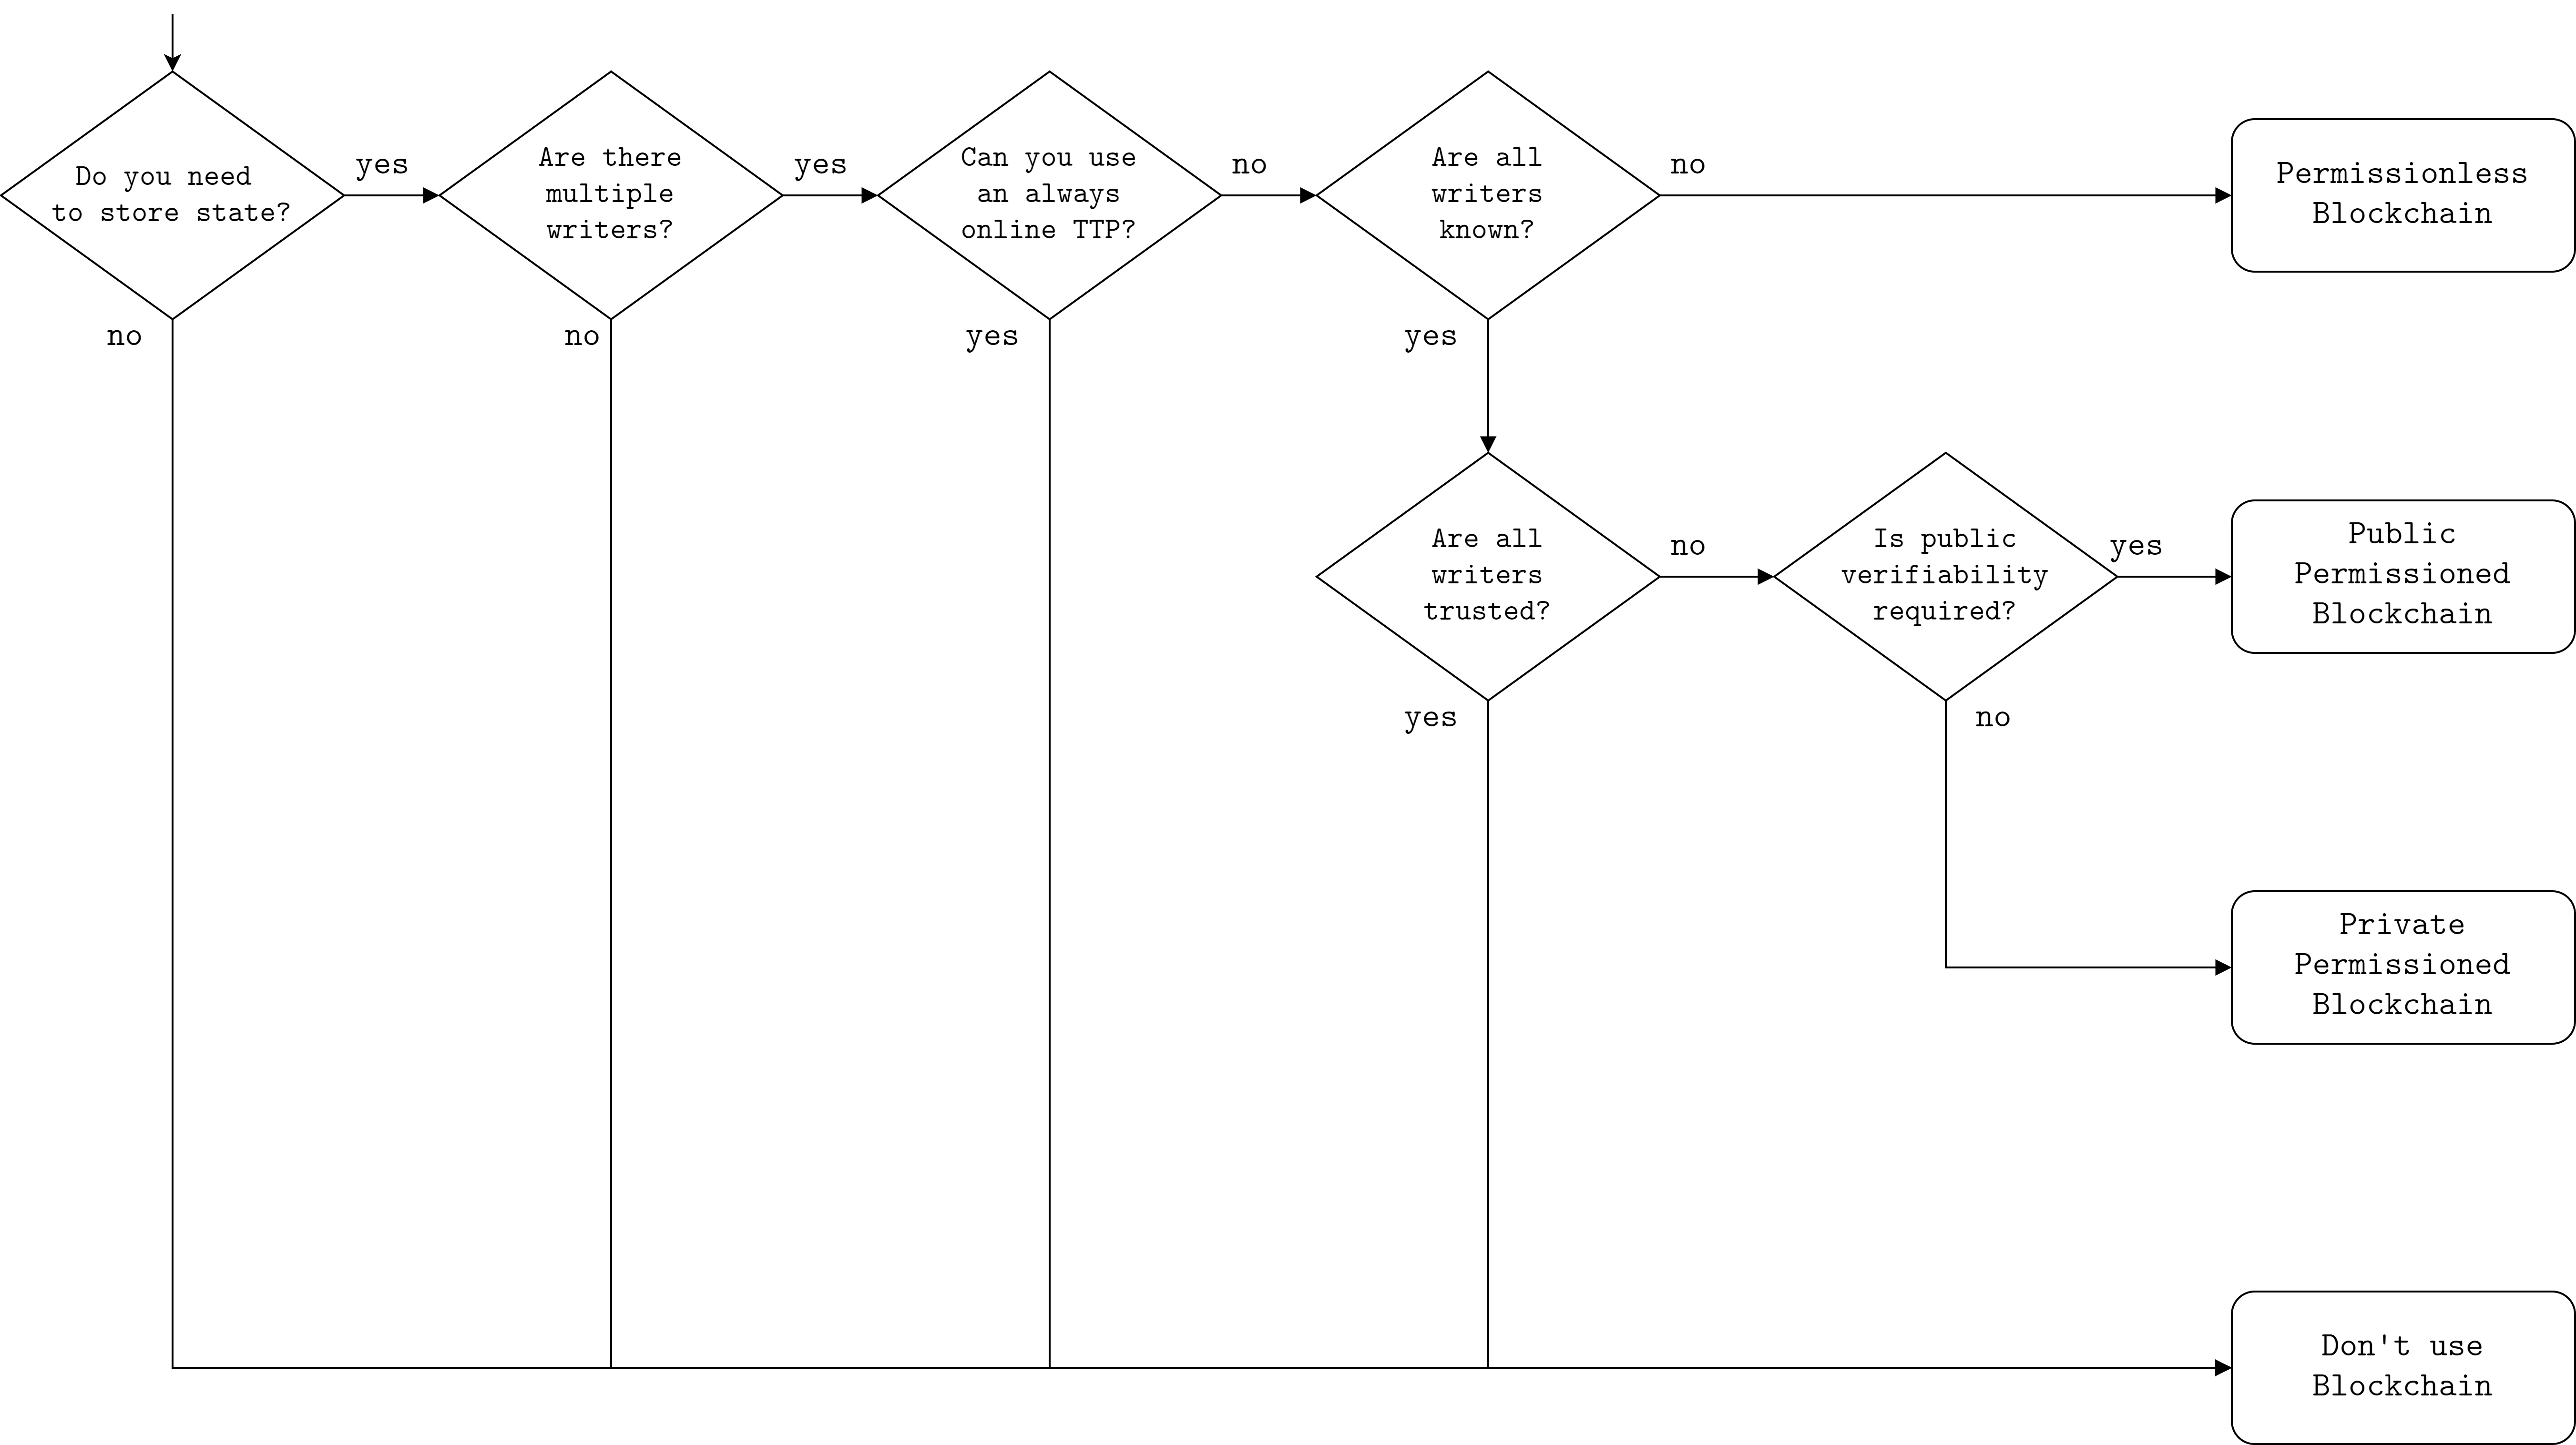
\includegraphics[width=12cm]{./Images/cap3/3.7.png}
\end{figure}

È possibile dividere idealmente le strutture basate su blockchain in tre livelli:
\begin{itemize}
    \item \textbf{Transaction Layer}: definisce il linguaggio di codifica e i criteri utilizzati durante la generazione di transazioni e smart contract. Entrambi devono essere firmati prima della loro diffusione per garantire il non ripudio e consentire il controllo dell'accesso e l'autenticazione del loro contenuto.
    \item \textbf{Block-Generation Layer}: sono presenti i processi di convalida delle transazioni e mining dei blocchi. Tutte le transazioni sono inserite in un blocco candidato, secondo regole di convalida. L'algoritmo di consenso viene adottato per garantire che tutti i nodi della rete abbiano una vista consistente dello stato della blockchain.
    \item \textbf{Distribution Layer}: ne fa parte il processo di distribuzione, così come l'inserimento del mined block nella blockchain. Tale inserimento riesce solo se l'hash del blocco estratto è corretto, altrimenti viene scartato. Al momento dell'inserimento di un blocco, lo stato globale della blockchain cambia e la vista globale della blockchain viene aggiornata.
\end{itemize}

\section{Il consenso nelle Blockchain}
In una rete blockchain, ogni partecipante può validare transazioni e proporre nuovi blocchi. L'obiettivo del protocollo di consenso nelle blockchain è di garantire che tutti i nodi partecipanti concordino sulla storia comune delle transazioni nella rete:
\begin{itemize}
    \item \textbf{Termination}: da ogni nodo onesto, una nuova transazione è sia scartata o accettata nella blockchain, all'interno del contenuto di un blocco.
    \item \textbf{Agreement}: ogni nuova transazione e il suo blocco che la contiene deve essere sia scartata o accettata da tutti i nodi onesti. Un blocco accettato deve avere lo stesso numero di sequenza per ogni nodo onesto.
    \item \textbf{Validity}: se ogni nodo riceve uno stesso blocco/transazione valida, esso deve essere accettato nella blockchain.
    \item \textbf{Integrity}: per ogni nodo onesto, tutte le transazioni accettate devono essere consistenti tra di loro (senza double spending). Tutti i blocchi accettati devono essere correttamente generati e collegati con hash in ordine cronologico.
\end{itemize}
Sono requisiti simili a quanto visto nel classico consenso distribuito: mentre \textbf{termination} e \textbf{validity} rappresentano la \textit{liveliness} del sistema, \textbf{agreement} e \textbf{integrity} rappresentano la \textit{safety} del sistema. 

Tuttavia l'agreement è potenziato con il total ordering, che rappresenta la serializzazione di blocchi e transazioni, mentre l'integrity impone la correttezza dell'origine di transazioni e blocchi, consentendo una protezione nei confronti del double spending e favorendo la \textit{tamper-proofing} nella blockchain.

\vspace{5mm}

Il teorema CAP si applica anche alle blockchain, con la relativa impossibilità di garantire entrambe le proprietà. Per i meccanismi di consenso, liveliness e safety hanno una diretta correlazione con il teorema: la \textbf{liveliness} garantisce che il processo di consenso completa sempre i suoi round. Anche se non si arriva a consenso, il meccanismo non attende indefinitamente, garantendo la sua availability. La \textbf{safety} garantisce che i suoi partecipanti siano nello stesso stato dopo un round, garantendo la consistenza nella rete.

Nei meccanismi di consenso delle blockchain si distinguono tre elementi chiave:
\begin{itemize}
    \item come vengono selezionati i partecipanti al consenso;
    \item come viene realizzato il processo di raggiungimento del consenso;
    \item come sono strutturati i dati nella blockchain.
\end{itemize}
Il protocollo di consenso si compone di cinque elementi:
\renewcommand{\theenumi}{\arabic{enumi}}
\begin{enumerate}
    \item la proposta di un blocco: generazione di blocchi e associazione di prove;
    \item la propagazione di informazioni: disseminazione di blocchi e transazioni nella rete;
    \item la validazione di blocchi: controllo dei blocchi per la generazione di prove e verifica della validità delle transazioni;
    \item la finalizzazione dei blocchi: raggiungimento del consenso sull'accettazione di blocchi validati;
    \item il meccanismo di incentivazione: promozione di partecipanti onesti e creazione di token di rete.
\end{enumerate}
Il consenso su blockchain si ispira al meccanismo di \textbf{State Machine Replication} (SMR).
\subsection{State Machine Replication}
SMR stabilisce i seguenti requisiti:
\begin{itemize}
    \item Tutti i server iniziano con lo stesso stato iniziale;
    \item Total order broadcast: tutti i server ricevono la stessa sequenza di richieste secondo l'ordine di generazione dai client;
    \item Tutti i server che ricevono la stessa richiesta emetteranno gli stessi risultati di esecuzione e termineranno nello stesso stato.
\end{itemize}
Sussiste una corrispondenza tra gli elementi del consenso nelle blockchain e quelli in SMR:
\begin{enumerate}
    \item La proposta di blocchi corrisponde alle richieste di operazioni da parte dei client in SMR e il leader che inizia il consenso;
    \item La propagazione delle informazioni corrisponde al reliable broadcast delle richieste di operazioni;
    \item La validazione dei blocchi corrisponde alla verifica delle firme e l'esecuzione delle operazioni richieste;
    \item La finalizzazione dei blocchi corrisponde al raggiungimento del consenso da parte dei server sullo stato corrente;
    \item Il meccanismo di incentivo non trova una corrispondenza. Questo perché SMR presuppone un gruppo ben definito di partecipanti che si presuppongono onesti.
\end{enumerate}
L'algoritmo di consenso di Paxos è uno schema SMR progettato per garantire il consenso tollerante a guasti di tipo crash: un proposer suggerisce un valore all'inizio e lo scopo del sistema è di far sì che gli acceptor concordano su un singolo valore e i learners apprendano tale valore dagli acceptor.

\begin{figure}[htb!]
    \centering
    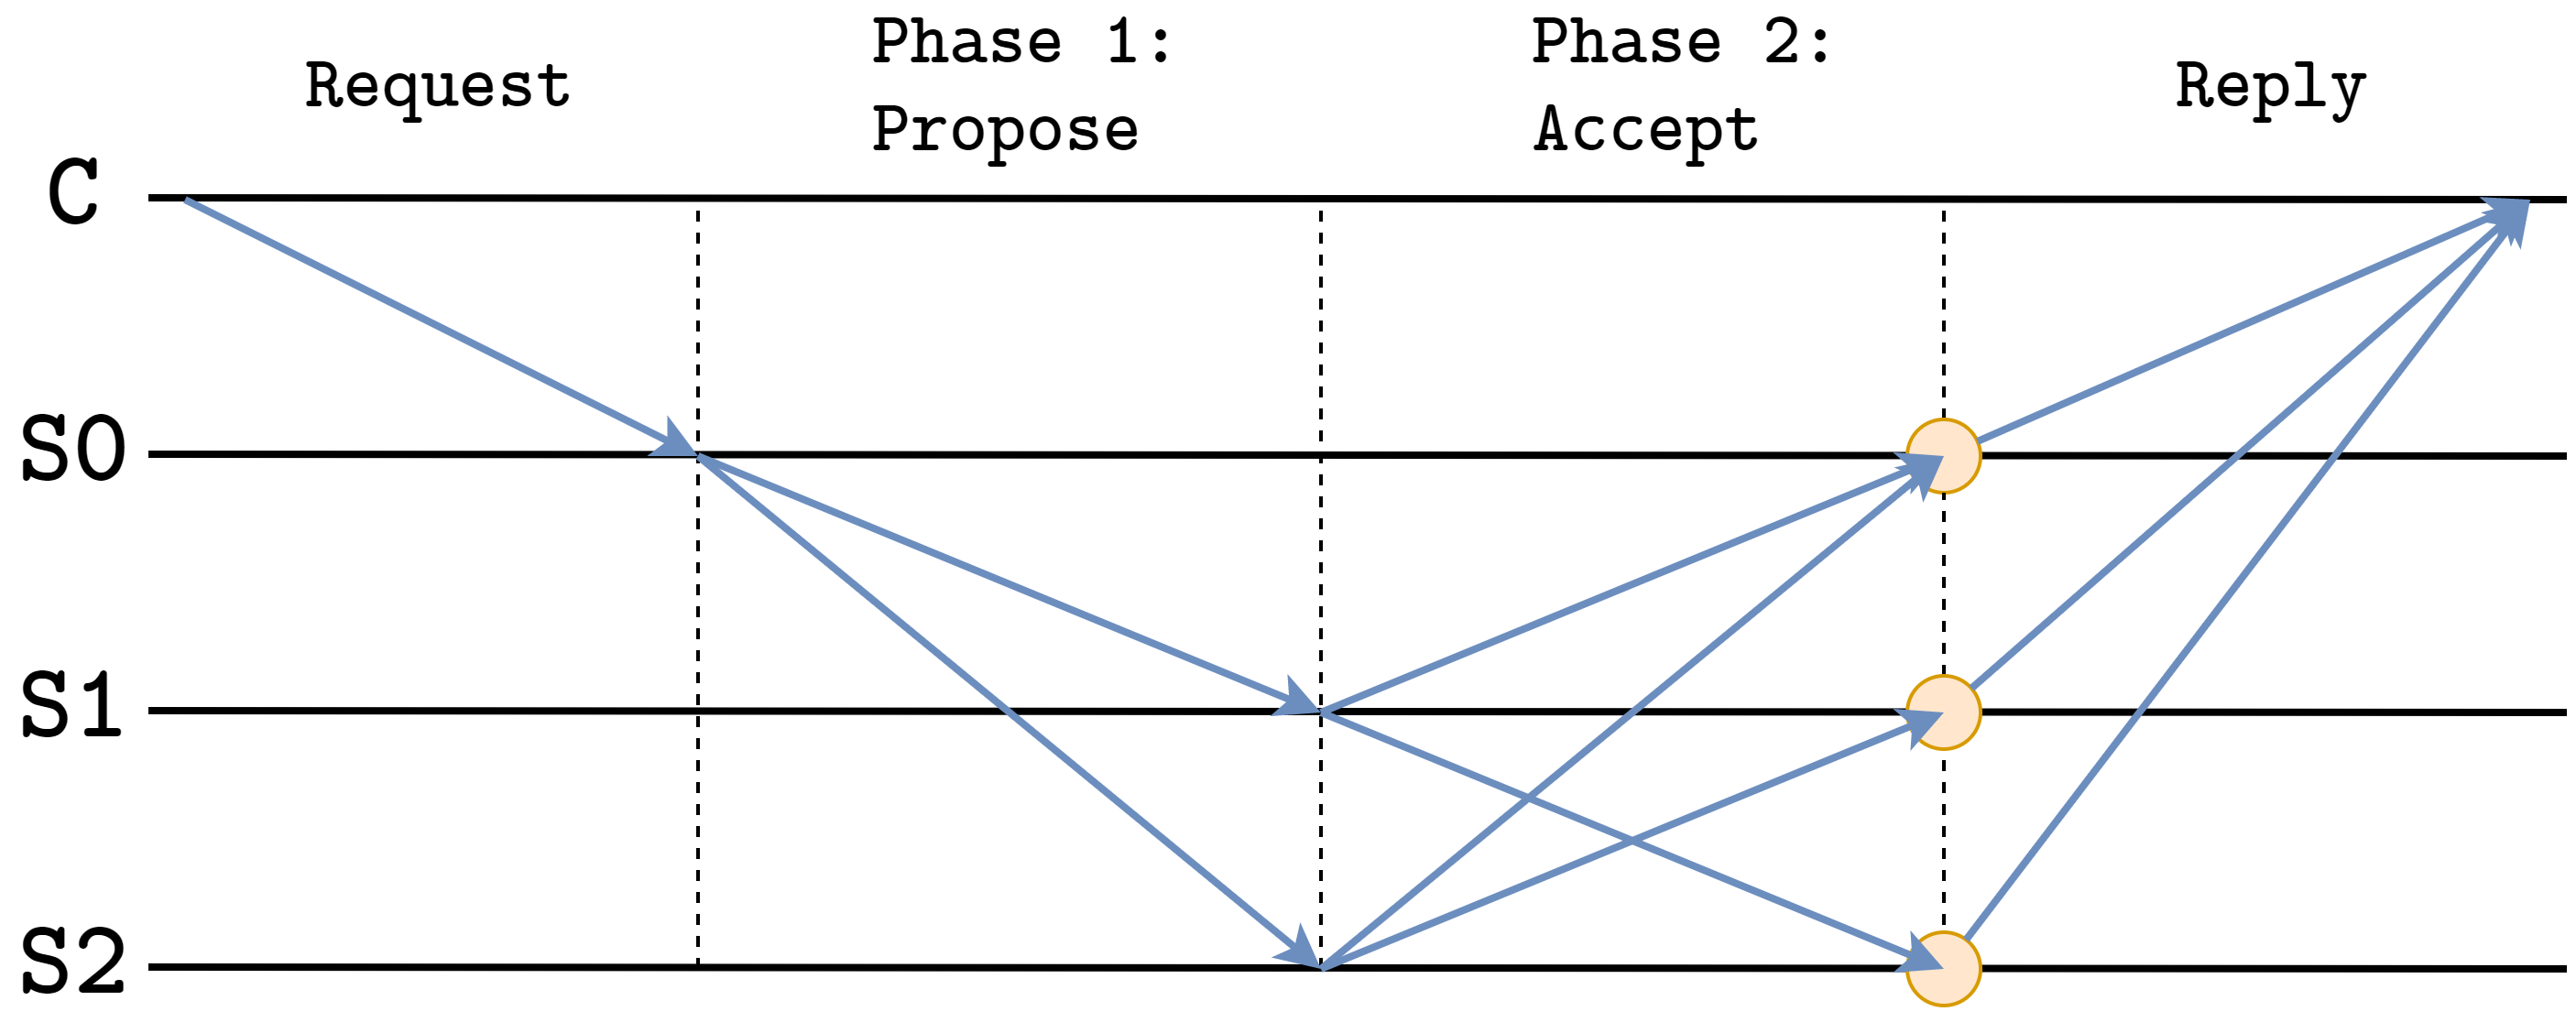
\includegraphics[width=9cm]{./Images/cap3/3.8.png}
\end{figure}

Come si può vedere dalla figura, il client è un learner e il leader tra i server è un proposer, mentre le repliche sono degli acceptors. Il client richiede il consenso su un singolo valore.

Il proposer propaga la richiesta agli acceptors, che si scambiano informazioni sui propri stati. Dopo essersi aggiornati allo stesso stato, tutti i server eseguono la richiesta e la inviano al client.

Il client riceve i risultati dagli acceptor e formula l'esito a maggioranza. Quando il leader è indisponibile per crash, le repliche ne eleggono uno nuovo.

Quest'algoritmo tollera \textit{f} crash dei server il cui numero \textit{N} è maggiore di \textit{2f + 1}, ma non tollera guasti bizantini.


\subsection{Pratical Byzantine Fault Tolerance}
L'algoritmo di PBFT è uno schema SMR che tollera i guasti bizantini ed è diventato sinonimo di tolleranza ai guasti bizantini nel contesto delle blockchain. Si compone di tre fasi:
\begin{itemize}
    \item Tutti i risultati inviati al client devono essere uguali, altrimenti il client decide a maggioranza. Il client invia una richiesta al nodo primario (leader), che la trasmette a tutti i nodi secondari (backup) assegnando un numero di sequenza.
    \item I nodi secondari e il leader si accordano sull'ordinamento delle richieste, e quando l'ordinamento è stato approvato la richiesta viene eseguita e un risultato viene restituito al client.
    \item Se il client ricevee \textit{f+1} risposte identiche, si raggiunge consenso.
\end{itemize}

\begin{figure}[htb!]
    \centering
    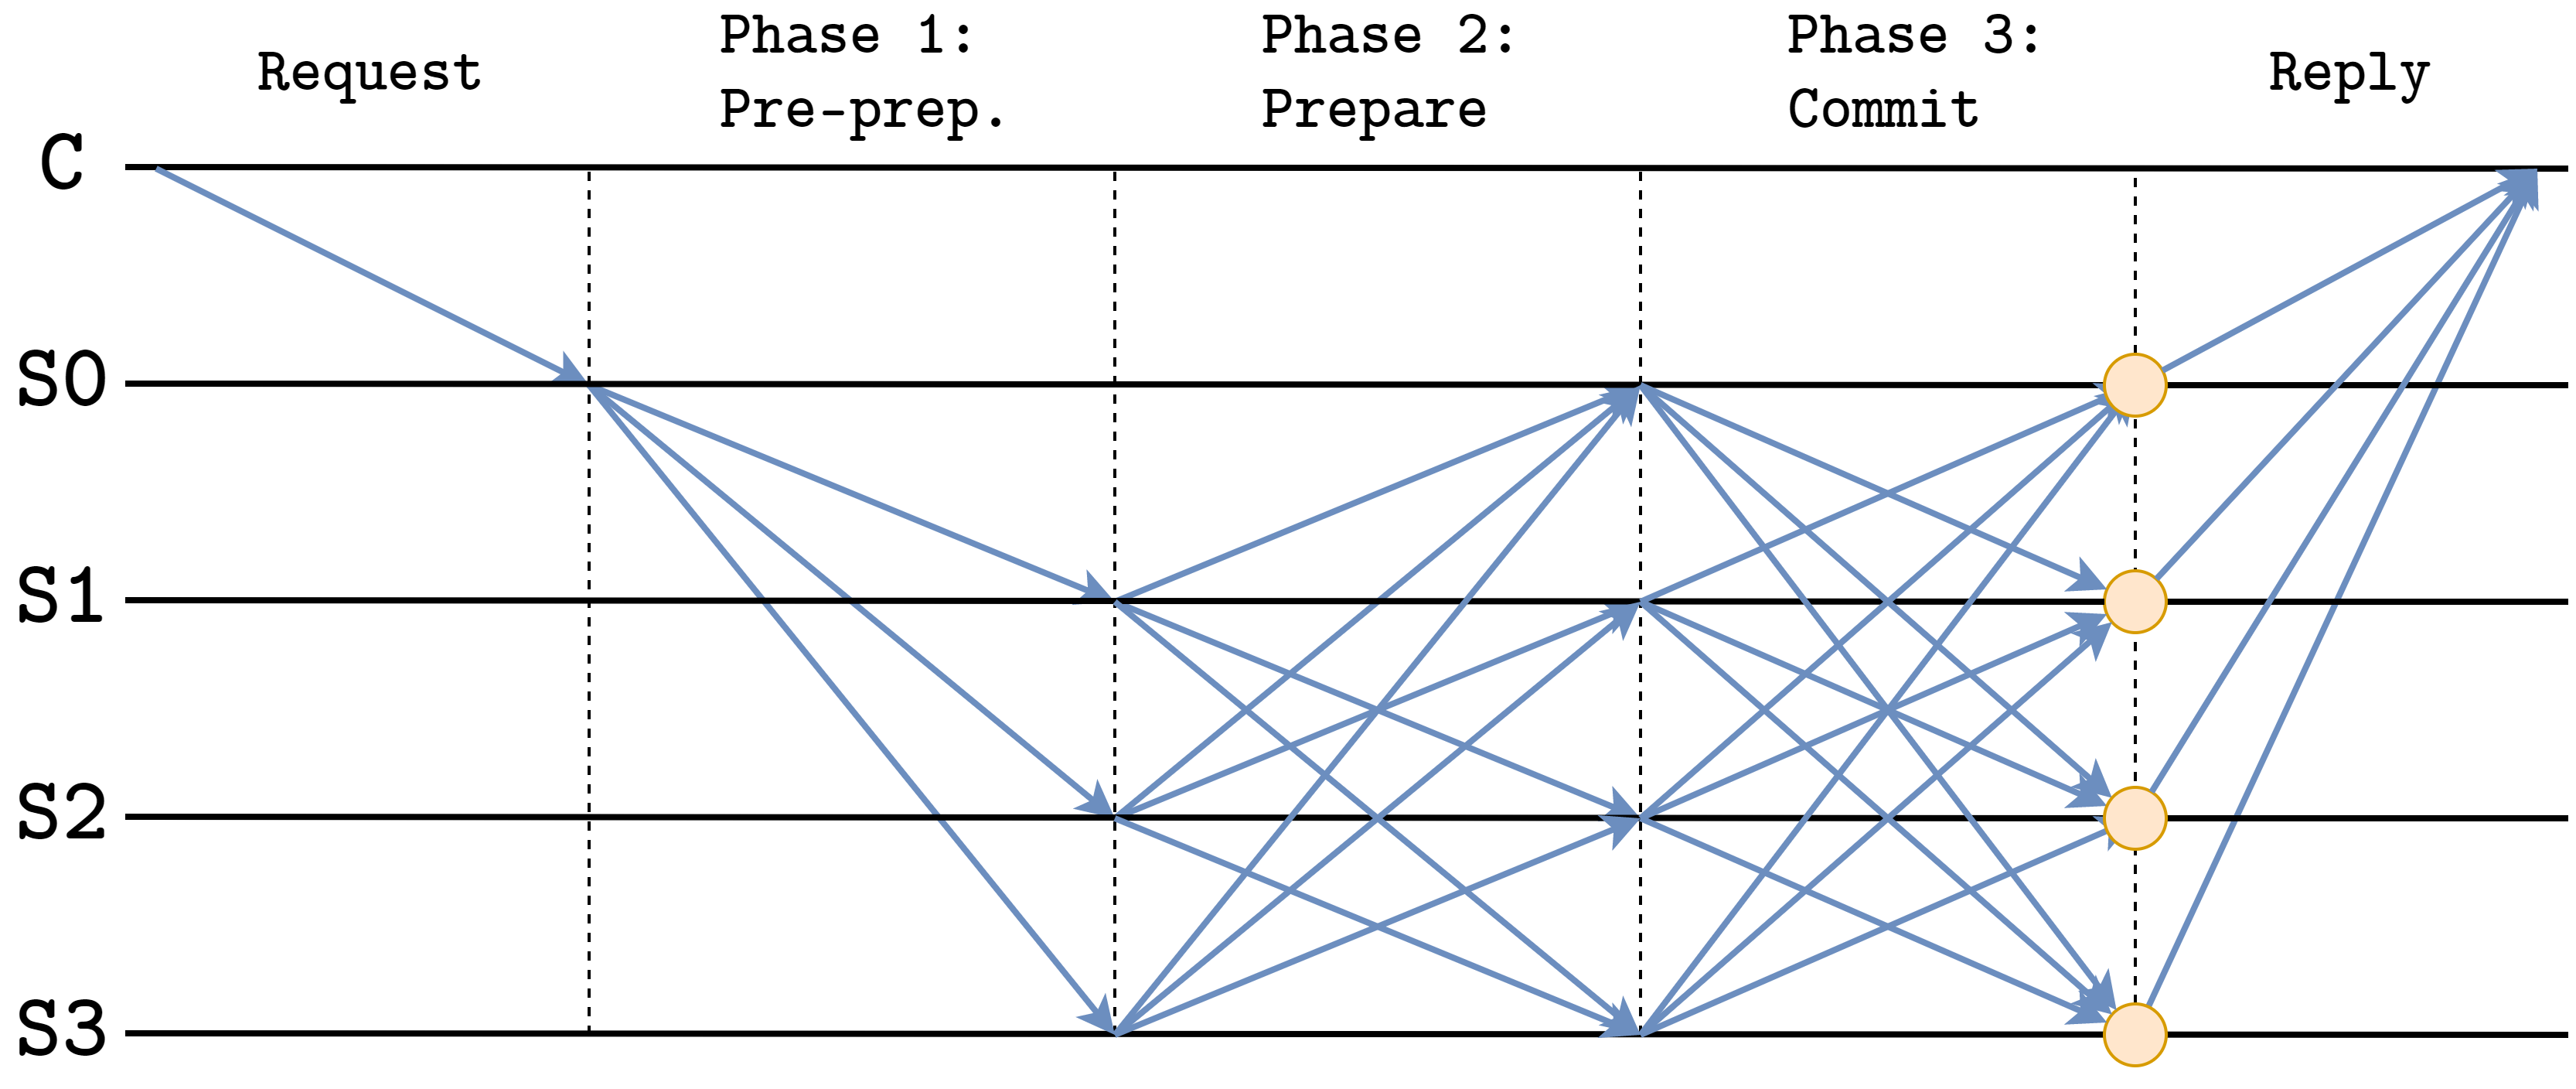
\includegraphics[width=10cm]{./Images/cap3/3.9.png}
\end{figure}

Il leader è scelto per ogni round dell'algoritmo o vista. I nodi sono ordinati in base al proprio identificativo, ed indicando il numero della vista con \textit{v} il leader è il modo con identificativo \textit{i = v mod N}.

Quando una replica nota un comportamento errato da parte del leader, se ne può richiedere la sostituzione con il meccanismo della \textit{view change} e l'elezione di un nuovo leader.

L'algoritmo consente di tollerare \textit{f} guasti anche di natura bizantina, con \textit{N} maggiore o uguale di \textit{3f + 1}, ovvero i nodi bizantini non riescono a far deviare il consenso raggiunto.

\vspace{5mm}

La primitiva di comunicazione alla base delle implementazioni PBFT nel contesto delle blockchain è il gossiping, impiegato per la propagazione di messaggi di blocchi o transazioni. A differenza della formulazione classica, nelle reti blockchain si ha la terminazione probabilistica: per ogni nodo onesto, ogni nuovo blocco è sia scartato o accettato nella sua blockchain locale. Un blocco accettato può essere ancora scartato ma con probabilità decrescente in maniera esponenziale con la crescita della dimensione della catena.

Il principale problema con la PBFT è che richiede che i nodi verifichino la validità dei messaggi degli altri e che il numero di nodi attivi in un dato momento sia sempre noto, e ciò lo rende applicabile in contesti \textit{permissioned}. Un altro svantaggio è che i leader vengono sostituiti solo quando le view change vengono attivate dalla rete. L'opportunità di diventare un leader è quindi unfair e mancano pochi incentivi per entrare a far parte della rete. Blockchain elegge i leader in base alla difficoltà del lavoro svolto, che genera incentivi, anche se spreca potenza di calcolo.

\vspace{5mm}

La sicurezza di PBFT si basa sul voto in tre fasi con MAC (Message Authentication Code) per la verifica dei messaggi. Sebbene non consumi molte risorse, di elaborazione, crea inevitabilmente problemi di scalabilità: in PBFT è impossibile espandersi oltre i 1000 nodi.

PBFT garantisce fortemente il requisito di \textit{safety}, perché una fork è quasi impossibile e viene garantita la terminazione immediata. Al contrario, la blockchain è più focalizzata sulla \textit{liveliness} che sulla safety: i fork si verificano abbastanza frequentemente (consenso multiplo) e affinché un blocco sia sicuro la sua catena deve essere più lunga di un certo numero di blocchi.

A tale scopo si è formulato un diverso algoritmo di consenso, quello di Nakamoto. Lo scopo è di evitare il consenso in gruppi chiusi, e di non punire i singoli nodi in gruppo aperto per essersi comportanti in modo malevolo, ma bisogna disincentivare i nodi a replicare comportamenti malevoli. A tal proposito, il processo di mining dei blocchi (ovvero calcolo della Proof of Work) è stocastico, per cui è impossibile sapere con certezza chi troverà la soluzione, anche se al crescere della difficoltà i nodi capaci di portare avvanti il processo diminuiscono. Questo scoraggia tutti gli agenti non disposti ad investire risorse economiche a partecipare al gioco.

Con il crescere dell'uso, e quindi del valore, la difficoltà a minare bitcoin aumenta, disincentivando ulteriormente chiunque voglia attaccare la rete. Inoltre, il crescente valore costringe gli agenti onesti ad investire di più nella sicurezza dei propri nodi, e di conseguenza della rete in generale. Le regole di validazione dei blocchi assicurano che nessun agente onesto accetti blocchi con informazioni scorrette.

\subsection{Il consenso Nakamoto}
Rispetto al consenso di Nakamoto implementato nel contesto della bitcoin, è possibile trovare un parallelismo con le 5 componenti del consenso nelle blockchain:
\begin{enumerate}
    \item La generazione di blocchi richiede una Proof of Work mediante la risoluzione di un puzzle crittografico con un determinato grado di difficoltà, tale da mantenere un intervallo di generazione e un grado di protezione adatti.
    \item Il gossiping viene impiegato per la distribuzione dei blocchi (transazioni appena ricevute o localmente generate=.
    \item Un blocco o transazione deve essere validata prima di essere inviata in broadcast agli altri o collegata alla coda di una catena locale. La validità si realizza evitando la double spending o controllando la PoW allegata al blocco.
    \item La catena più lunga rappresenta il raggiungimento del consenso in caso di disaccordo (che ha causato la fork).
    \item Chi ha generato un blocco accettato con successo può ottenere un reward o premio. Sottomettere una nuova transazione ha un costo monetario.
\end{enumerate}
L'impiego di PoW intensive è necessario per evitare e tollerare attacchi Sybil, a causa della natura \textit{permissionless} e pseudonima di alcune reti blockchain. Un attaccante può facilmente ottenere delle nuove identità, ma la risoluzione di una PoW implica il consumo di risorse di hash, che può essere difficilmente falsata. La reward per i blocchi e il costo delle transazioni serve ad incentivare i nodi a partecipare onestamente.

\vspace{5mm}

Nelle classiche formulazioni del consenso distribuito, le caratteristiche di tolleranza ai guasti è espressa in termini di numero di nodi non corretti che si possono tollerare. Nel caso del consenso di Nakamoto è caratterizzata in termini di percentuale di potenza di hashing avversaria tollerabile.

Se la rete si sincronizza più velocemente del tasso di proposta di blocco basato su PoW, una maggioranza onesta può garantire il consenso su una parte stabile in continua crescita della blockchain. Fintanto che meno del 50\% della potenza di hashing totale è controllata in modo malizioso, i blocchi prodotti da miners onesti vengono propagati tempestivamente, la catena principale è della maggioranza onesta che eventualmente supera qualsiasi ramo malizioso.

Dal punto di vista del consenso distribuito classico, il consenso di Nakamoto elude abilmente il vincolo fondamentale di BFT pari a 1/3 adottando finalità probabilistiche. Nel consenso del BFT classico se più di 1/3 della popolazione è malizioso, i nodi onesti finiranno per decidere valori contrastanti, portando al fallimento del consenso. Nel consenso di Nakamoto, tuttavia, le decisioni contrastanti sono consentite temporaneamente sottoforma di fork della blockchain, a condizione che alla fine verranno eliminate dal continuo sforzo della maggioranza onesta.
Il consenso di Nakamoto soffre di alcune limitazioni, primo tra tutti un basso throughput delle transazioni. Si può dimostrare che l'intervallo di 10 minuti tra la generazione di blocchi garantisce che ogni nuovo blocco sia sufficientemente propagato prima che venga inserito nel sistema un nuovo blocco. Ridurre l'intervallo tra i blocchi aumenta il throughput delle transazioni, ma lascia i nuovi blocchi non sufficientemente propagati e provoca più incidenti di fork, minando la sicurezza della catena principale.

Aumentare la dimensione del blocco (attualmente a 1 MB) ha lo stesso effetto, poiché dimensioni maggiori portano a ritardi di trasmissione più elevati e una propagazione insufficiente. Inoltre, il meccanismo di PoW di Nakamoto causa enorme consumo di energia: una transazione Bitcoin in media consuma 431 KWh di elettricità.

\subsubsection{\textbf{ATTACCO ECLISSE}}
Se un potente attacco riesce a dominare la comunicazione in entrata/uscita tra un miner vittima e la rete principale, allora  la vittima non sarà più in grado di contribuire all'estensione della catena principale. Se il potere dell'attaccante è $\alpha$, allora un attacco double spending è possibile se $\alpha + \epsilon > 50\%$, con $\epsilon$ percentuali di miners eclissati.

L'attacco Eclisse è un exploit della debole connettività di una rete peer-to-peer senza autorizzazione basata su Internet. Per risolvere bisogna aumentare la connettività e la diversità geografica delle connessioni peer-to-peer.

\subsubsection{\textbf{SELFISH MINING}}
Se un gruppo di miners maligni trattiene i blocchi appena estratti e li pubblicizza strategicamente per interrompere la propagazione dei blocchi estratti da miner onesti, può parzialmente annullare il lavoro di miner onesti e amplificare il loro potere di estrazione.

Quando forma per la prima volta la sua catena segreta, il minatore egoista corre un rischio. Se ha generato il primo blocco segreto e poi un altro minatore ha generato un blocco, non può pubblicare il suo blocco segreto e avere la catena più lunga: si ha una corsa tra due rami di lunghezza 1. Il miner egoista cercherà di estendere il proprio ramo come tutti gli altri miner. Se vince, pubblica la catena più lunga, e l'attacco riparte. Se vincono gli altri, il miner egoista è in svantaggio.

A prima vista potrebbe sembrare che l'attacco non funzioni: il miner di minoranza perderà più gare di quante ne vince. Tuttavia, il grafico seguente mostra che non è così in generale. Un insieme di selfish miner più grande di 1/3 della potenza di mining aumenterebbe le sue entrate deviando dal protocollo prescritto ed eseguendo \textit{selfish mining}.

\begin{figure}[htb!]
    \centering
    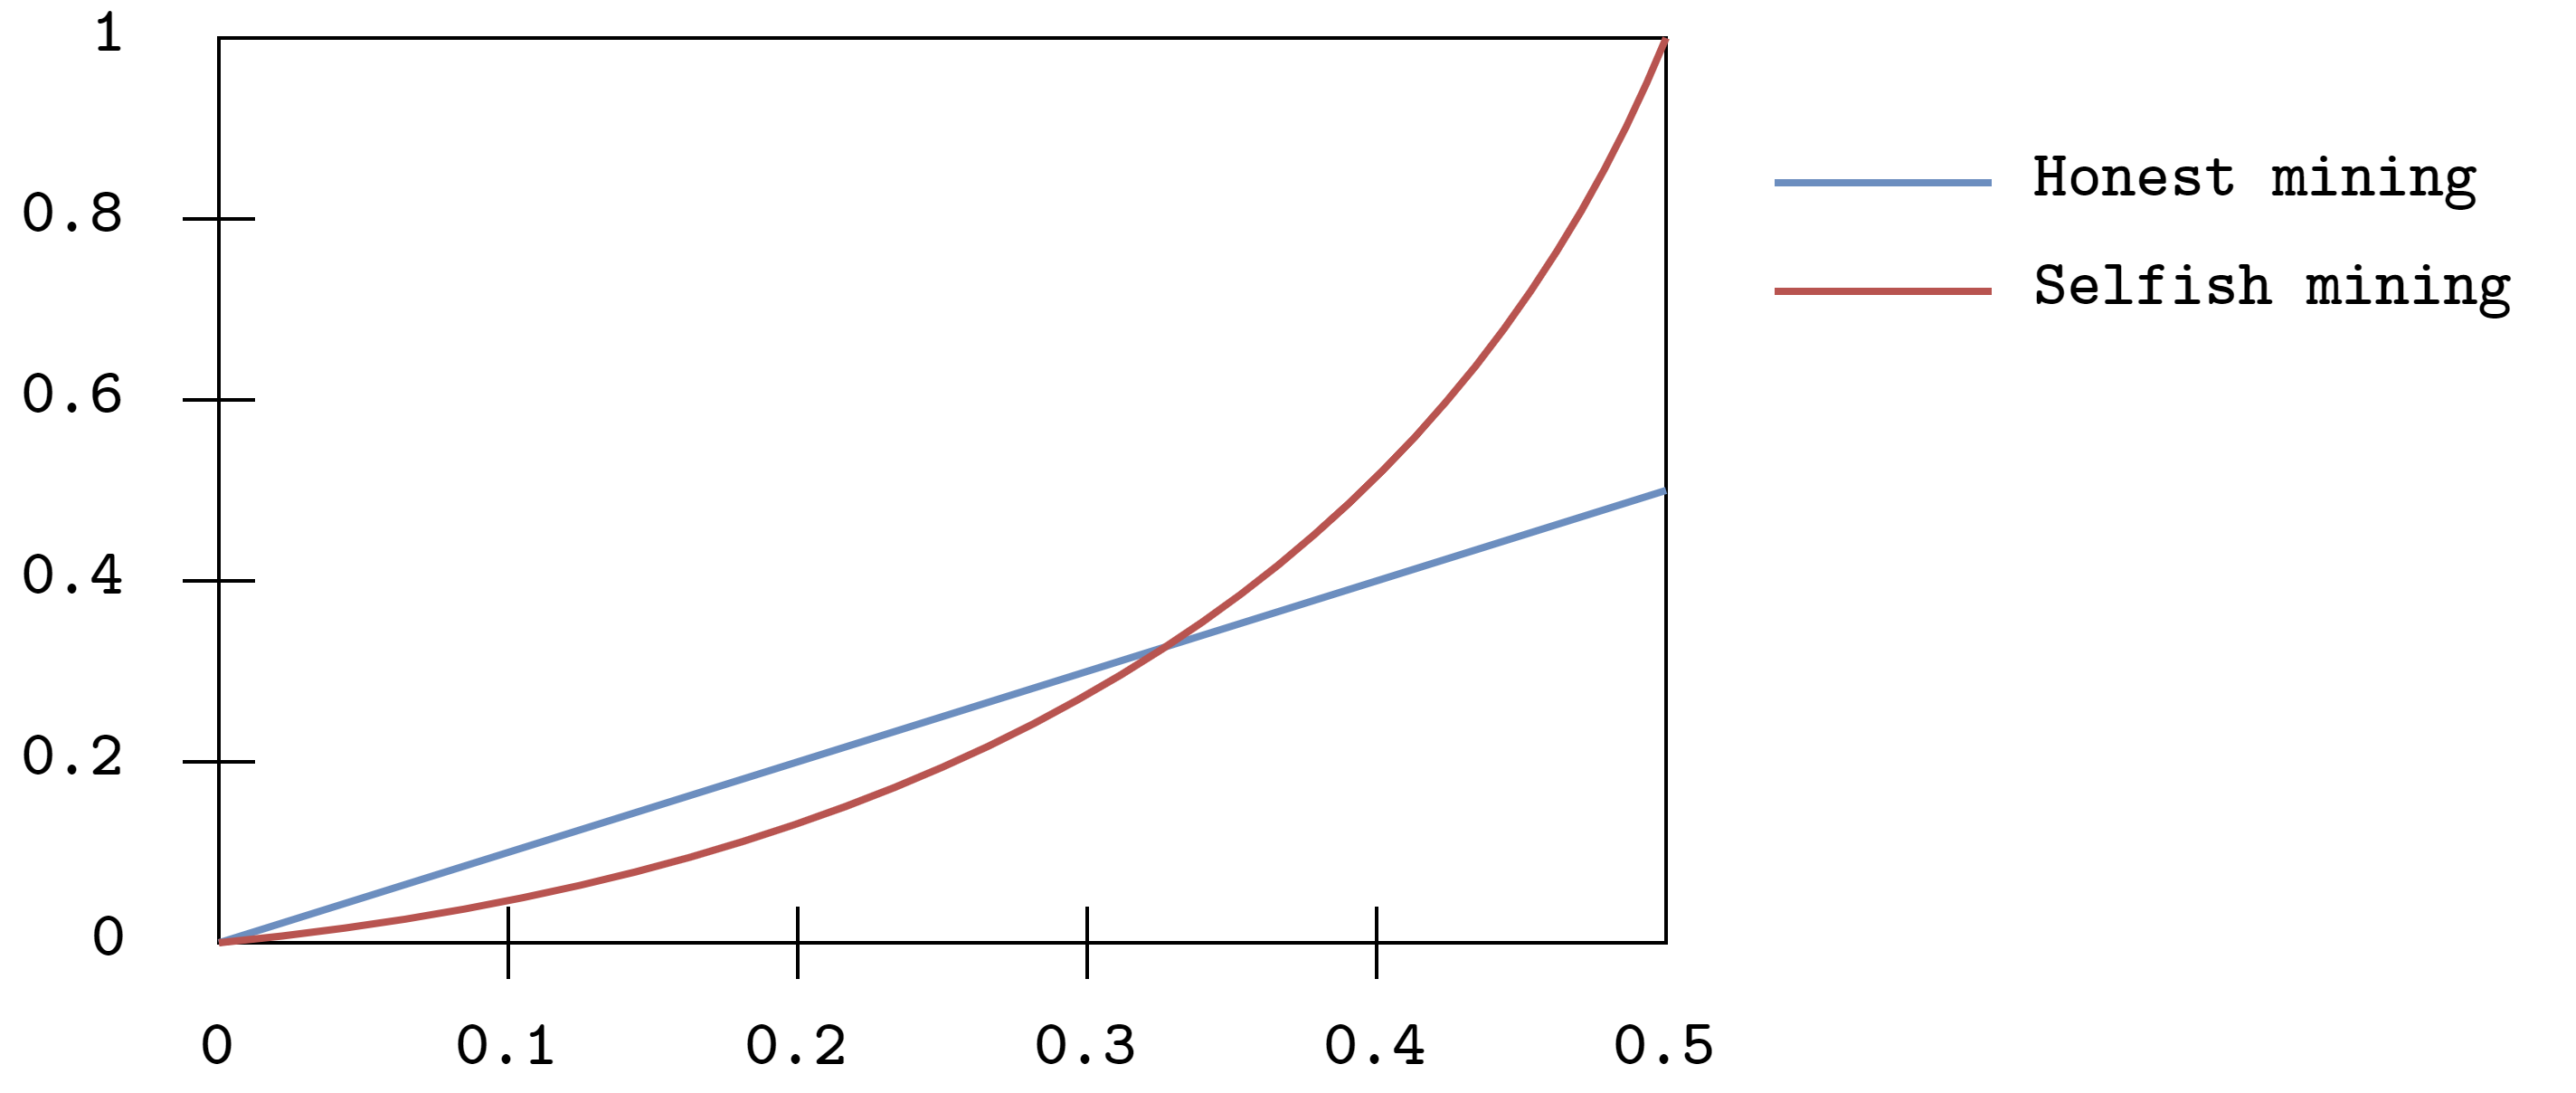
\includegraphics[width=10cm]{./Images/cap3/3.10.png}
\end{figure}

\subsection{Proof of Stake}
È un'alternativa efficiente dal punto di vista energetico al PoW. Uno Stake (puntata) si riferisce alle monete o token posseduti da un partecipante che possono essere investiti nel processo di consenso. Rispetto a PoW, la cui possibilità di proporre un blocco è proporzionale alla sua potenza di calcolo, la possibilità di proporre un blocco per PoS è proporzionale al valore del suo stake.

PoS non si basa sull'hashing dispendioso per generare blocchi, Poiché la difficoltà dell'hashing puzzle diminuisce con il valore dello stake del miner, il numero atteso di tentativi di hashing per un miner per risolvere il puzzle può essere significativamente ridotto se il suo valore di stake è alto. Pertanto, PoS evita la competizione di hashing brute force che si verificherebbe se fosse stato usato PoW, ottenendo così una significativa riduzione del costo computazionale.

\begin{figure}[htb!]
    \centering
    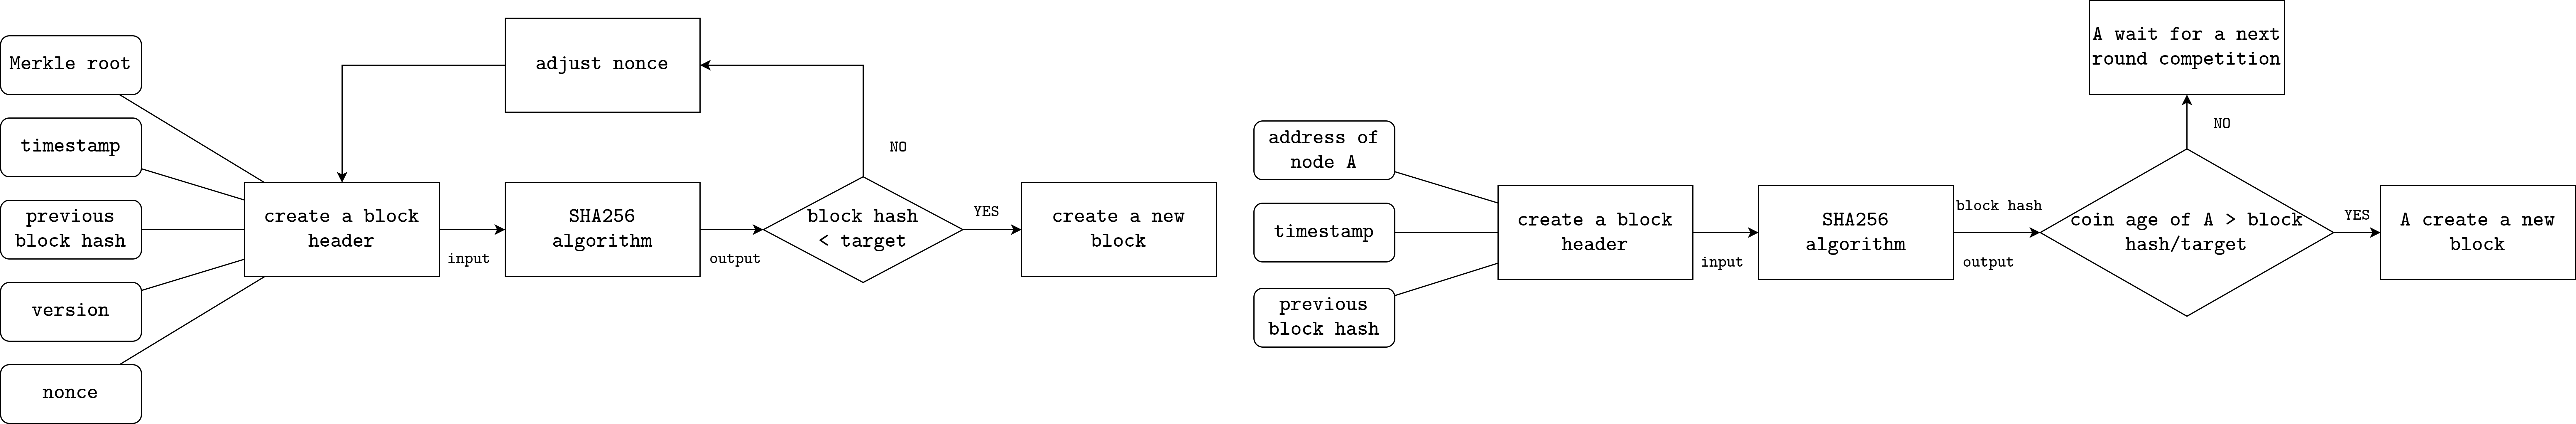
\includegraphics[width=15cm]{./Images/cap3/3.11.png}
\end{figure}

Questo implica l'assenza del premio per chi inserisce il blocco giusto nella blockchain, e del mining, in quanto non vengono create nuove unità di criptovaluta con la creazione di ogni blocco. I validatori sono ricompensati con una commissione per le transizioni validate. 

Una variante di PoS è la \textbf{Proof of Stake Delegato} (DPoS): consente ai nodi che detengono lo stake maggiore di votare per eleggere i verificatori di blocchi. Questo fa sì che i detentori di stake concedano il diritto di creare blocchi ai delegati che sostengono invece di creare blocchi stessi, riducendo così il loro consumo di potenza computazionale a 0.

\begin{figure}[htb!]
    \centering
    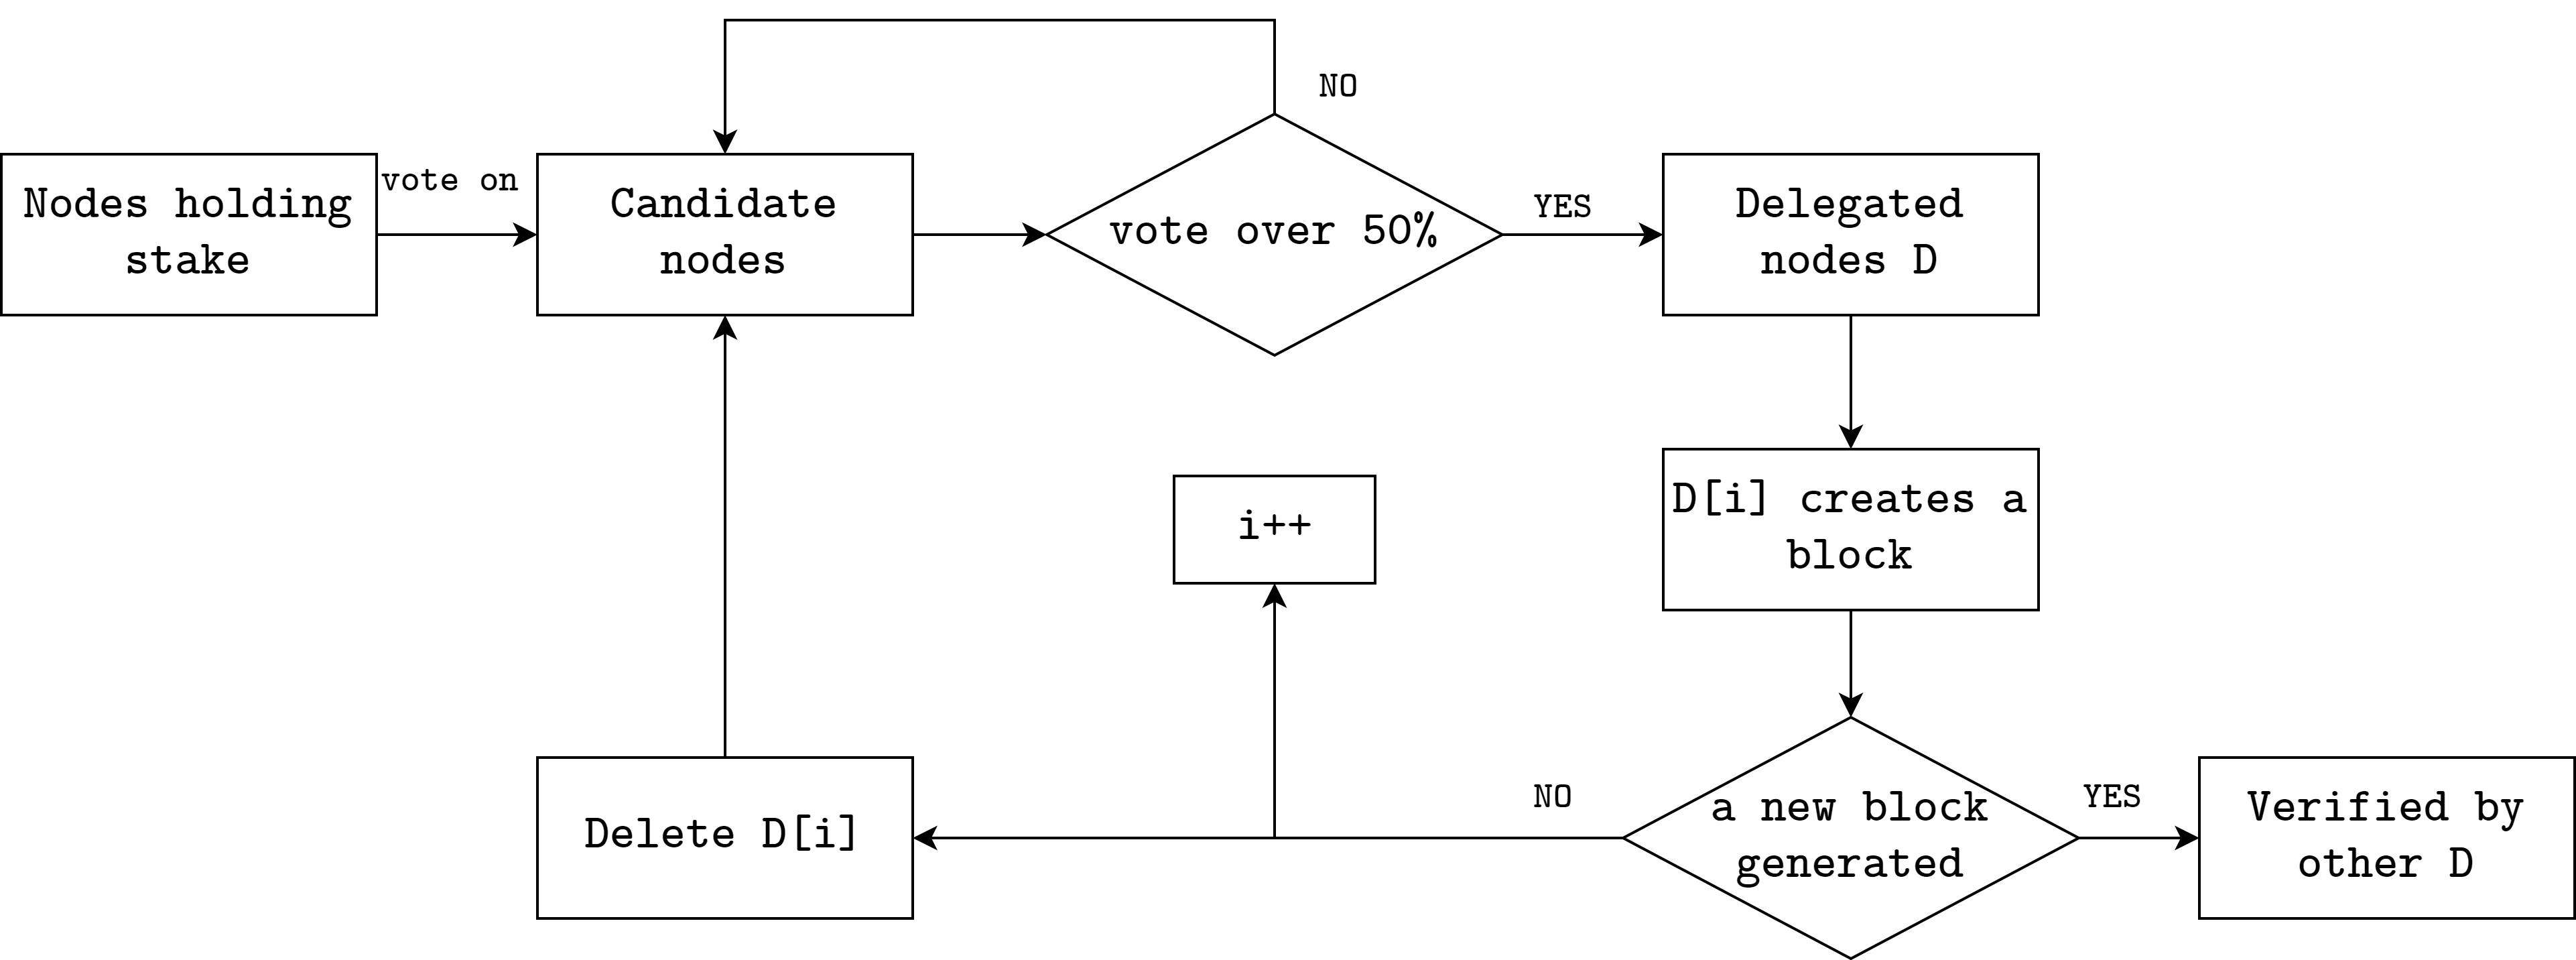
\includegraphics[width=10cm]{./Images/cap3/3.12.png}
\end{figure}

Mentre PoW avvantaggia i miners che hanno investito maggiormente in hardware, PoS dà un'influenza sproporzionata a coloro che posseggono un numero importante di criptovalute, con il rischio di un accentramento di ricchezza nelle mani di pochi, secondo il dogma secondo cui \textit{rich people get richer}.

Un altro problema è il \textit{nothing at stake}, per il quale nel caso di una fork del network i validatori saranno incentivati ad operare su entrambe le catene, risultando eventualmente in problemi di double spending. Questo problema è meno evidente in un sistema di DPoS.

PoS e DPoS sono stati applicati nel contesto di classici algoritmi BFT, come PBFT, al fine di consentirne l'applicazione in contesti open e \textit{permissionless}.

\subsection{Tendermint}
È un algoritmo di consenso ispirato a PBFT che sfrutta la PoS per il consenso in un ambiente permissioned, dove il gruppo dei validatori è un gruppo chiuso e precostituito. Ogni nuovo blocco viene validato o meno in una interazione dell'algoritmo, che si compone di molti round per poter giungere a consenso. Si tratta di un consenso di tipo CP, dove la consistenza viene fortemente garantita.

\begin{enumerate}
    \item Inizialmente, viene scelto a caso un validatore che propone un nuovo blocco;
    \item Il nuovo blocco viene distribuito agli altri validatori che ne verificano la validità e ne votano l'accettazione;
    \item Se sono arrivati i 2/3 dei voti ed oltre allora si conferma la decisione e si passa ad un'altra iterazione con un nuovo validatore, altrimenti si realizza un nuovo round;
    \item Ricordiamoci che essendo un algoritmo sincrono, si smette di aspettare dopo che è trascorso un timeout.
\end{enumerate}
Non tutti i validatori avranno lo stesso peso, ma la PoS viene usata per dare peso maggiore a chi ha uno stake maggiore. La condizione di 2/3 non è sul numero di votanti ma sulla quantita di criptovaluta totale nel sistema.

\vspace{5mm}

Per i meccanismi di consenso, liveliness e safety hanno una diretta correlazione con il teorema CAP:
\begin{itemize}
    \item La liveliness garantisce che il processo di consenso completa sempre i suoi round. Anche se non si arriva a consenso, il meccanismo non attende indefinitamente, garantendo la sua availability.
    \item La safety garantisce che i suoi partecipanti sono nello stesso stato dopo un round, garantendo così la consistenza nella rete.
\end{itemize}
Nelle reali implementazioni di soluzioni blockchain, non è mai possibile ottenere sia consistenza che availability, perché devono affrontare la tolleranza alle partizioni. Il sistema restituirà un errore o un timeout se non è possibile garantire che particolari informazioni siano aggiornate a causa del partizionamento di rete.

Tra le due opzioni rimanenti, i sistemi di tipo permissioned in un gruppo chiuso di nodi scelgono di privilegiare di garantire la consistency anziché l'availability, perché non sono focalizzate su criptovalute ma sulla gestione di dati in ambito distribuito.


\section{Smart Contracts}
Un contratto è un accordo legalmente vincolante che riconosce e disciplina i diritti e i doveri delle parti del contratto. Uno smart contract è la trasposizione in codice di un contratto. È un programma deterministico che elabora le informazioni in una blockchain: a parità di input i risultati restituiti saranno identici. Uno smart contract per blockchain deve soddisfare i seguenti obiettivi: osservabilità, verificabilità, riservatezza e applicabilità. Su una blockchain, uno smart contract non può essere modificato, ma può facilmente essere osservato e verificato. Il ciclo di vita di uno smart contract può essere sintetizzato come segue:
\begin{enumerate}
    \item Gli sviluppatori scrivono la logica per lo smart contract in un linguaggio di programmazione supportato dalla piattaforma blockchain che desiderano utilizzare. Utilizzando un compilatore specifico (di solito fornito dalla piattaforma stessa) compilano il codice sorgente del loro smart contract e ottengono una sua rappresentazione in bytecode.
    \item Lo smart contract è pubblicato sulla piattaforma blockchain ed archiviato. Una volta pubblicato, sarà di sola lettura o modificabile. Nel caso in cui sia di sola lettura, per fornire un aggiornamento gli sviluppatori dovranno pubblicare una nuova versione dello smart contract e reindirizzare gli utenti ad essa. Una volta caricato, lo smart contract è al suo stato iniziale, pari ai valori iniziali delle variabili interne.
    \item L'accesso a un programma di smart contract pubblicato dipende dalla piattaforma blockchain, come un indirizzo restituito quando lo smart contract è caricato nella piattaforma. Tale indirizzo può essere utilizzato per interagire con lo smart contract, inviando le transazioni contenenti la funzione che desiderano utilizzare e gli argomenti della funzione. Se è necessaria una quantità di valuta della piattaforma per avviare l'esecuzione della funzione, tale importo sarà trasferito insieme alla transazione. La transazione verrà archiviata nel pool di transazioni della piattaforma blockchain che attendono di essere eseguite e convalidate.
    \item La piattaforma blockchain selezionerà le transazioni da eseguire e convalidare. Durante l'esecuzione, le funzioni nella transazione verranno eseguite dai nodi. Durante la validazione, i nodi confronteranno i propri risultati e selezioneranno quello da mantenere secondo un protocollo di consenso.
    \item Una volta selezionato il risultato valido, verrà inserito in un blocco da aggiungere alla blockchain. Se una transazione validata ha alterato le variabili interne di uno smart contract, i nuovi valori saranno considerati come valori iniziali da transazioni future sullo smart contract.
\end{enumerate}
L'implementazione di smart contract non è standardizzata e ogni piattaforma propone una propria soluzione. Le funzioni di uno smart contract possono essere chiamate direttamente dal client o indirettamente da altri smart contracts. Per garantire che le chiamate terminino, al client viene addebitata una fee ad ogni chiamata e sua durata. Se l'addebito supera quello che il cliente è disposto a pagare, il calcolo viene interrotto e le operazioni annullate.


L'attuale approccio di sviluppo di smart contract limita il throughput perché non ammette concorrenza. Quando un miner crea un blocco, assembla una sequenza di transazioni e calcola un nuovo stato provvisorio eseguendo gli smart contract di tali transazioni in serie, nell'ordine in cui si verificano nel blocco. Un miner non può eseguire gli smart contracts in parallelo, perché potrebbero sussistere degli accessi in conflitto a dati condivisi e un interleaving arbitrario potrebbe produrre uno stato finale non coerente. Spesso per gli smart contracts non è possibile dire in anticipo se le esecuzioni di contratti siano in conflitto.


\section{Principali piattaforme}

\subsection{Bitcoin}


Bitcoin utilizza il modello UTXO (Unspent Transaction Output). Ogni transazione è identificata da un certo numero di bitcoin in ingresso e in uscita. In ingresso, si ha l'indirizzo delle transazioni mai usate in precedenza e la cui somma degli output equivale all'output della transazione che le contiene. I destinatari di una transazione sono identificati da un indirizzo Bitcoin, un identificatore di 26-35 caratteri. Gli indirizzi possono essere generati gratuitamente da qualsiasi utente.

Spesso è difficile avere transazioni che sommate risultino esattamente pari alla quantità da trasferire. L'eccedenza deve essere trasferita all'autore della transazione. Il modello UTXO non permette di ritrovare sulla blockchain il saldo corrente di un determinato utente, che deve essere ricostruito raccogliendo tutte le transazioni che presentano un determinato utente in output e quelle con tali transazioni in input. UTXO consente transazioni parallele perché non esiste alcun account, inoltre consente l'anonimato dal momento che un utente può disporre di multipli indirizzi Bitcoin. Essendo stateless, rende complesso la realizzazione di applicazioni come smart contracts, ma permette di ottenere resilienza ed elasticità, oltre che la possibilità per qualsiasi istanza di eseguire qualsiasi attività.

I multipli indirizzi Bitcoin di un utente fungono da pseudonimi per garantire la privacy, e si suole impiegare un indirizzo per ogni transazione. Un modo ingenuo per accettare pagamenti in Bitcoin è dire ai propri clienti di inviare denaro a un determinato indirizzo. Essendo le transazioni Bitcoin pubbliche, se Alice invia Bitcoin, un utente malizioso Bob potrebbe vedere tale transazione e inviare una e-mail affermando che è stato l'autore del pagamento: il destinatario del pagamento non è in grado di distinguere se il trasferimento è stato effettivamente svolto da Bob o Alice, per questo motivo si usa indicare un indirizzo per ogni cliente che deve effettuare un pagamento.

\vspace{5mm}

È possibile impiegare una transazione conoscendo il suo identificativo, che è pubblico. Sorge il problema di evitare che utenti maliziosi impieghino transazioni che non sono proprie, e per formulare dei meccanismi di controllo di autenticazione della legittimità di utilizzo, è stato realizzato un sistema di scripting su Bitcoin, precursore degli smart contract.

\textbf{Script} è un semplice programma imperativo, basato su stack ed elaborato da sinistra a destra:
\begin{itemize}
    \item Uno script è essenzialmente un elenco di istruzioni registrate con ogni transazione che descrivono come la prossima persona che desidera spendere i Bitcoin trasferiti può accedervi.
    \item Una transazione è valida se nulla genera un errore e l'elemento in cima allo stack è \texttt{true} alla fine dello script.
    \item Gli stack contengono vettori di byte.
\end{itemize}
Il linguaggio di scripting ha due tipi di istruzioni: 
\begin{itemize}
    \item Le istruzioni di dati contengono semplicemente un valore e sono racchiuse tra parentesi angolari (\texttt{$<data>$}).
    \item Gli \texttt{OP CODE} sono operazioni specifiche appartenenti al linguaggio Bitcoin Scripting che agisce sul valore in cima allo stack e pone il loro risultato anche in cima allo stack.
    \item Nell'immagine successiva è possibile vedere tre output diversi:
    \begin{itemize}
        \item Per spendere il primo output, è necessario fornire due numeri la cui somma è 8.
        \item Per spendere il secondo output, vanno fornite due diverse stringhe di dati che producono lo stesso risultato hash.
        \item Per spendere il terzo output, va dato qualcosa che ha lo stesso hash di ciò che è all'interno del blocco.
    \end{itemize}
\end{itemize}

\begin{figure}[htb!]
    \centering
    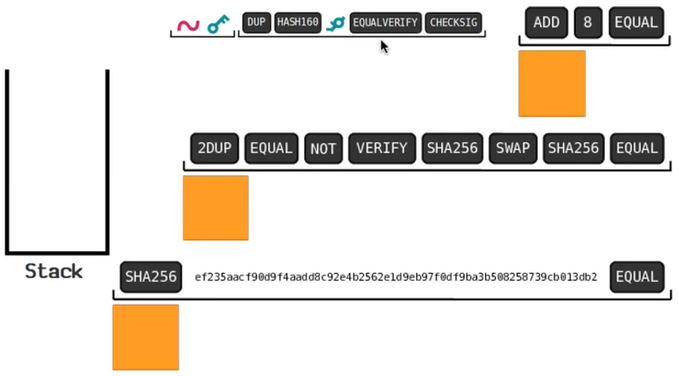
\includegraphics[width=8cm]{./Images/cap3/3.13.png}
\end{figure}

Ogni codice operativo ha una corrispondente rappresentazione esadecimale, che viene usata per fornire la sua codifica. Uno \textit{locking script} viene posizionato su ogni output creato in una transazione, mentre è necessario fornire uno \textit{unlocking script} per ogni input che si desidera spendere in una transazione. Anche se l'unlocking script è fornito dopo il locking script iniziale, in realtà viene messo per primo quando si eseguono entrambi gli script.

Il linguaggio non è Turing-completo: non ci sono istruzioni condizionali e cicli, perché si vuole predicibilità dei tempi di esecuzione, che dipende deterministicamente dal numero di istruzioni in esse contenute. Inoltre è senza stato, non hanno informazione della valuta sbloccata, o non accede alle informazioni del blocco che li contiene.



Alcune caratteristiche di Bitcoin:
\begin{itemize}
    \item \textbf{Throughput}: mediamente 7tps (transactions per second), contro le 2000tps di VISA e 5000tps di Twitter
    \item \textbf{Latency}: 10 minuti per completare una transazione (contro i pochi secondi di VISA)
    \item \textbf{Size and bandwidth}: ogni blocco è almeno 1MB (con un throughput ai livelli di visa si avrebbero circa 214 PB all'anno)
    \item \textbf{Security}: sensibile ad attacchi di tipo 51\%
    \item \textbf{Wasted resources}: a casusa della competizione generata dalla Proof of Work
    \item \textbf{Usability}: API complesse per l'utilizzo al di fuori dell'ambito Bitcoin
    \item \textbf{Scalability}: ad ogni passo la blockchain aggiunge un ulteriore blocco, ogni blocco aumenta con i dati rappresentativi dei precedenti. Man mano che un maggior numero di utenti si unisce alla rete e i blocchi aumentano, il sistema rischia di deformarsi
    \item \textbf{Privacy}: ogni nodo conosce le transazioni eseguite dagli altri, in quanto deve verificarne la validità. Vengono utilizzati degli pseudonimi per garantire la privacy degli utenti
\end{itemize}
Strettamente legato alla tecnologia blockchain è il concetto di \textbf{Smart Contract}. Gli smart contract sono applicazioni che facilitano, verificano o fanno rispettare la negoziazione o l'esecuzione di un contratto. Uno smart contract si presenta in forma di codice che risiede e viene eseguito direttamente all'interno della catena. Tramite gli smart contract può avvenire una trasposizione "informatica" di accordi che si concludono al di fuori della piattaforma tecnologica, mediante funzioni \texttt{if/then} incorporate in software o protocolli informatici.

\begin{mdframed}[backgroundcolor=gray!20,shadow=false]
\textbf{Esempio di applicazione in campo assicurativo}
\begin{itemize}
    \item \textbf{L'ACCORDO} - Due parti stipulano un contratto (come una polizza assicurativa), traducendo e registrando i dettagli in uno smart contract. Ad esempio, clausole su particolari aspetti: le condizioni e gli effetti indesiderati (il rimborso in caso di ritardo del volo aereo).
    \item \textbf{LA VERIFICA} - Lo smart contract viene quindi inserito (trascritto) nella blockchain (come Ethereum, che è pubblica e permissionless), registrato e reso esecutivo dall'insieme dei partecipanti (nodi + miners) sulla base di parametri concordati. C'è un controllo sulla disponibilità dei fondi dell'utente che registra il contratto.
    \item \textbf{IL BLOCCO} - La rete dei dispositivi interconnessi garantisce il mantenimento, l'accessibilità e il corretto aggiornamento di un registro condiviso (ledger). Lo smart contract entra a far parte di un blocco (identificato da un codice hash) che viene validato dai partecipanti alla blockchain.
    \item \textbf{IL MINING} - In Ethereum il meccanismo di validazione è quello del Proof of Work, la soluzione di un enigma matematico connesso al codice del blocco. Il miner che trova la soluzione e registra il contratto ottiene una remunerazione: una fee (da parte di chi sottopone il contratto: più alta l'offerta, più veloce la registrazione) e un premio corrisposto creando nuova moneta (in questo caso Ether).
    \item \textbf{LA CATENA} - Una volta validato, cioè ottenuto il consenso dei nodi, il blocco (con una marca temporale, timestamp) viene aggiunto alla catena, immutabile e certificata. L'operazione è pubblica e mostrata nella piattaforma. Ogni nodo aggiunge il blocco alla catena: la sequenza degli hash crea una catena sicura e non contraffabile.
    \item \textbf{L'ORACOLO} - La blockchain non può accedere a dati esterni alla rete (come gli orari di arrivo degli aerei), interviene quindi l'oracolo: un agente terzo (come un'applicazione) che passa informazioni allo smart contract appena la condizione esterna si verifica (ritardo del volo). L'oracolo può essere un singolo o un "comitato" di attori, per ridurre la centralizzazione.
    \item \textbf{L'ESECUZIONE} - Ricevuto l'input dell'oracolo, scatta automaticamente la clausola \texttt{if/then}. Lo smart contract tra le parti si autoesegue: se l'orario del volo supera il ritardo tollerato dall'accordo, scatta il rimborso dell'assicurato.
\end{itemize}
\end{mdframed}

\subsection{Ethereum}
È la più grande piattaforma software decentralizzata (open source) che consente lo sviluppo di smart contracts e applicazioni decentralizzate senza entità di terze parti. Si tratta di una blockchain potenziate da un linguaggio di programmazione incorporato. Questi contratti possono essere utilizzati in maniera sicura per eseguire un vasto numero di operazioni: sistemi elettorali, registrazione di domini, mercati finanziari, ecc.

La valuta digitale gestita è l'\textbf{Ether}. Ogni operazione richiede una commissione, chiamata \textbf{gas}: è il carburante necessario per svolgere una determinata operazione. Il costo del gas è espresso in \textbf{wei} (10\textsuperscript{-18} Ether).

\vspace{5mm}

Una \textbf{transazione} è un messaggio firmato che esegue un'operazione associata alla blockchain. Nel caso di \textit{cryptocurrency} si tratta di inviare una certa quantità di valuta ad altri nodi della rete. In altri casi possono essere considerate le transazioni le azioni come la registrazione dei nomi di dominio, la realizzazione e l'adempimento delle offerte commerciali e la stipula dei contratti.

\vspace{5mm}

Lo \textbf{stato} è un set di dati di cui una blockchain network deve rigorosamente tenere traccia e che rappresenta i dati attualmente rilevanti per le applicazioni implementate sulla catena. Lo stato è costituito da una serie di oggetti definiti \textit{accounts}. L'esecuzione di una transazione comporta un cambiamento di stato.

Ethereum gestisce due diversi tipi di account:
\begin{itemize}
    \item \textbf{Externally owned accounts} (EOA), che sono in grado di inviare e ricevere Ether, e inviare transazioni agli smart contract.
    \item \textbf{Contract accounts}, che oltre alle funzionalità degli EOA hanno del codice associato e le loro azioni vengono triggerate da EOA o altri contract accounts. L'esecuzione del codice modifica le informazioni contenute nel proprio spazio di archiviazione (consente di utilizzare la blockchain per scopi diversi dalla cryptocurrency).
\end{itemize}
I contratti hanno generalmente quattro scopi:
\begin{enumerate}
    \item gestire un data store che rappresenti qualcosa di utile per altri contratti o per il mondo esterno;
    \item comportarsi come un EOA con politiche di accesso più complicate (una sorta di filtro che consente l'inoltro di messaggi a determinate EOA solo se determinate condizioni vengono soddisfatte);
    \item gestire un contratto o una relazione in corso tra più utenti (un esempio è un contratto che paga automaticamente chi invia una soluzione valida ad alcuni problemi matematici, o dimostra che sta fornendo una risorsa computazionale);
    \item fornire funzionalità ad altri contratti (una sorta di libreria).
\end{enumerate}
Gli smart contracts sono solitamente scritti in linguaggi di programmazione di alto livello (ad es. Solidity), e tale codice viene compilato dalla Ethereum Virtual Machine (EVM) e deployato nella blockchain sottoforma di \textit{EVM bytecode}. L'EVM consente a chiunque di eseguire l'EVM bytecode.


Come per Bitcoin, anche nel caso di Ethereum il consenso nella versione 1.0 è basato su PoW, con l'intento di migrare verso PoS. L'algoritmo utilizzato è \textbf{Ethash}: tale algoritmo consente di calcolare la PoW in maniera più veloce rispetto alla soluzione adottata da Bitcoin. Per aumentare la complessità del problema da risolvere si agisce sulla memoria piuttosto che sul costo computazionale. Ethash utilizza un algoritmo di hash appartenente alla famiglia Keccak, la stessa delle funzioni hash SHA-3. Utilizza un set di dati di grandi dimensioni che viene periodicamente rigenerato e cresce lentamente nel tempo.

Svolge una serie di intensive letture ad accesso casuale in memoria al set di dati di 2 GB strutturato come un grafo aciclico diretto (DAG). La risoluzione si realizza con 64 cicli a partire dall'hash di informazioni di partenza con pagine estratte dal DAG. Il digest viene confrontato con una soglia target. Se inferiore o uguale, il calcolo è considerato riuscito. In caso contrario, l'algoritmo viene rieseguito con un nonce diverso (incrementando quello corrente o scelgliendone uno nuovo a caso).

\vspace{5mm}

Gli indirizzi EOA cominciano con il prefisso \texttt{0x} seguito dai 20 byte più a destra dell'hash della chiave pubblica. Gli indirizzi di contratto sono nello stesso formato, ma sono determinati dal mittente e dal nonce pari al numero di transazione inviato dal cliente.

Ethereum non si basa sugli output di transazione non spesi (UTXO), ma gli account hanno uno stato che indica il saldo corrente. Lo stato non è memorizzato sulla blockchain, ma in un albero separato di Merkle. Un wallet di criptovaluta memorizza le chiavi pubbliche e private (un utente può avere più indirizzi), che possono essere utilizzati per ricevere o spendere ether. I wallet sono come applicazioni che consentono di interagire con un account Ethereum, analogamente alle app di e-banking di un conto bancario.

I contratti hanno generalmente 4 scopi:
\begin{itemize}
    \item gestire un data store che contiene informazioni utili per altri contratti o per il mondo esterno:
    \item comportarsi come un EOA con politiche di accesso più avanzate (una sorta di filtro che consente l'inoltro di "messaggi" a determinate EOA solo se determinate condizioni vengono soddisfatte);
    \item gestire o un contratto o una relazione in corso tra più utenti (un esempio è un contratto che paga automaticamente chi invia una soluzione valida ad alcuni problemi matematici, o dimostra che sta fornendo una risorsa computazionale);
    \item fornire funzionalità ad altri contatti (una sorta di libreria).
\end{itemize}
Il codice viene interpretato dalla Ethereum Virtual Machine (EVM) e rappresentato in EVM bytecode. Gli account dei contratti sono diversi:

% \usepackage{colortbl}


\begin{table}[htb!]
\centering
\begin{tabular}{|c|c|c|} 
\hline
\multicolumn{1}{|l|}{}                                                                                                                          & Account personale      & Account di contratto                                                           \\ 
\hline
{\cellcolor[rgb]{1,0.584,0}} \textcolor{white}{address}  & H(pub\_key)            & H(addr + nonce del creatore)                                                   \\ 
\hline
{\cellcolor[rgb]{1,0,0.4}}\textcolor{white}{code}                                                                                               & $\varnothing$             & \begin{tabular}[c]{@{}c@{}}Codice\\\textcolor[rgb]{0.4,0,0.6}{} \end{tabular}  \\ 
\hline
{\cellcolor[rgb]{0.831,0,1}}\textcolor{white}{storage}                                                                                          & $\varnothing$              & Dati                                                                           \\ 
\hline
{\cellcolor[rgb]{0,0.298,1}}\textcolor{white}{balance}                                                                                          & Saldo ETH (in Wei)     & Saldo ETH (in Wei)                                                             \\ 
\hline
{\cellcolor[rgb]{0,0.663,0.78}}\textcolor{white}{nonce}                                                                                         & \# transazioni inviati & \# transazioni inviati                                                         \\
\hline
\end{tabular}
\end{table}

\begin{itemize}
    \item \textbf{from} - Indirizzo dell'utente di origine della transazione.
    \item \textbf{signature} - Firma della nuova transazione usando la chiave privata dell'utente creatore.
    \item \textbf{to} - Indirizzo dell'utente di destinazione della transazione.
    \item \textbf{amount} - Quantità di ETH trasferita.
\end{itemize}

Nel caso di transazioni per smart contracts la struttura cambia per contenere anche i dati per il contratto:

\begin{table}[htb!]
\centering
\begin{tabular}{lllll}
{\cellcolor[rgb]{1,0.635,0}}~ ~\textcolor{white}{from~ ~} & {\cellcolor[rgb]{1,0,0.408}}~\textcolor{white}{signature~} & {\cellcolor[rgb]{0.827,0,1}}~ ~ \textcolor{white}{to~ ~~} & {\cellcolor[rgb]{0.012,0.384,0.988}}~ ~\textcolor{white}{amount~ ~} & {\cellcolor[rgb]{0,0.502,0.502}}\textcolor{white}{~ ~ data~ ~~} 
\end{tabular}
\end{table}

Di seguito è mostrato uno snippet di bytecode che  mostra una transazione EOA to EOA.

\begin{lstlisting}[escapeinside={(*}{*)}]
(*\texttt{> web3.fromWei(eth.getBalance(eth.accounts[0]))}*)
(*\texttt{100}*)
(*\texttt{> web3.fromWei(eth.getBalance(eth.accounts[1]))}*)
(*\texttt{100}*)
(*\texttt{> eth.sendTransaction\{}*)
      (*\texttt{from: eth.accounts[0],}*)
      (*\texttt{to: eth.accounts[1],}*)
      (*\texttt{value: web3.toWei(10)}*)
(*\texttt{"0x497913c178f656197264f8864c836vbc74bcb44532c352d }*)
(*\texttt{>}*)
(*\texttt{> web3.fromWei(eth.getBalance(eth.accounts[0]))}*)
(*\texttt{89.99958}*)
(*\texttt{> web3.fromWei(eth.getBalance(eth.accounts[1]))}*)
(*\texttt{110}*)
\end{lstlisting}

Il comando \texttt{Web3.fromWei} consente di convertire il Ether un valore espresso in Wei, mentre \texttt{Web3.toWei} fa il contrario. Come si può osservare la transazione ha richiesto una commissione (gas), per cui il valore associato ad \texttt{accounts[0]} è inferiore a 90 Ether. L'avvenuta transazione genera un codice di hash come ricevuta.


% \usepackage{colortbl}


\begin{table}[hbt!]
\centering
\begin{tabular}{|c|c|c|} 
\hline
\rowcolor[rgb]{0.902,0.902,0.902}                                                                                                                                       & \textbf{Bitcoin}                                           & \textbf{Ethereum}                                                          \\ 
\hline
{\cellcolor[rgb]{0.902,0.902,0.902}}\textbf{Utilizzo}                                                                                                                   & \begin{tabular}[c]{@{}c@{}}\\Cryptocurrency\\\end{tabular} & \begin{tabular}[c]{@{}c@{}}Cryptocurrency +~\\smart contract\end{tabular}  \\ 
\hline
{\cellcolor[rgb]{0.902,0.902,0.902}}\textbf{Modello}                                                                                                                    & \begin{tabular}[c]{@{}c@{}}\\UTXO\\\end{tabular}           & Account/Balance                                                            \\ 
\hline
{\cellcolor[rgb]{0.902,0.902,0.902}}\begin{tabular}[c]{@{}>{\cellcolor[rgb]{0.902,0.902,0.902}}c@{}}\textbf{Tempo per la creazione}\\\textbf{di un blocco}\end{tabular} & 10 minuti                                                  & 10/12 secondi                                                              \\ 
\hline
{\cellcolor[rgb]{0.902,0.902,0.902}}\textbf{Nascita}                                                                                                                    & \begin{tabular}[c]{@{}c@{}}\\Genesis block\\\end{tabular}  & Presale                                                                    \\
\hline
\end{tabular}
\end{table}
\clearpage

\textbf{Solidity} è un linguaggio di programmazione con tipizzazione statica ed orientato agli oggetti per la scrittura di applicazioni che implementano la logica di busineess incorporata in smart contract su Ethereum e altre piattaforme blockchain. È progettato attorno alla sintassi ECMAScript ma si differenzia per una tipizzazione statica e tipi di ritorno variadici. Supporta inoltre tipi complessi definiti dall'utente, ad esempio struct ed enumerazioni, che consentono di raggruppare i tipi di dati correlati. I contratti supportano l'ereditarietà, inclusa quella multipla con linearizzazione C3. È stata inoltre introdotta un'interfaccia binaria dell'applicazione (ABI) che facilita più funzioni type-safe all'interno di un singolo contratto.

\begin{mdframed}[backgroundcolor=gray!20,shadow=false]

La linearizzazione C3 è un algoritmo utilizzato per ottenere l'ordine in cui i metodi devono essere ereditati in presenza di ereditarietà multipla. La linearizzazione è la somma della classe più un merge delle linearizzazioni dei suoi genitori e un elenco dei genitori stessi. Il merge viene eseguito selezionando la prima intestazione delle liste che non appare nella coda di nessun'altra. L'elemento selezionato viene rimosso e aggiunto all'elenco di output. Se non è possibile selezionare un'intestazione valida, allora l'unione è impossibile da calcolare a causa di ordinamenti incoerenti delle dipendenze e nessuna linearizzazione è possibile.

\texttt{L(O) := [O]}

\texttt{L(A) := [A] + merge(L(O),[O]) = [A] + merge([O],[O]) = [A, O]}

\texttt{L(K1) := [K1] + merge(L(A),L(B),L(C),[A,B,C]) + [K1] + merge([A,O],[B,O],[V,O],}

\texttt{[A,B,C]) = [K1,A] + merge([O],[B,O],[C,O],[B,C]) = [K1,A,B] + merge([O],[O],}

\texttt{[C,O],[C]) = [K1,A,B,C] + merge([O],[O],[O]) = [K1,A,B,C,O]}

\end{mdframed}

\begin{figure}[htb!]
    \centering
    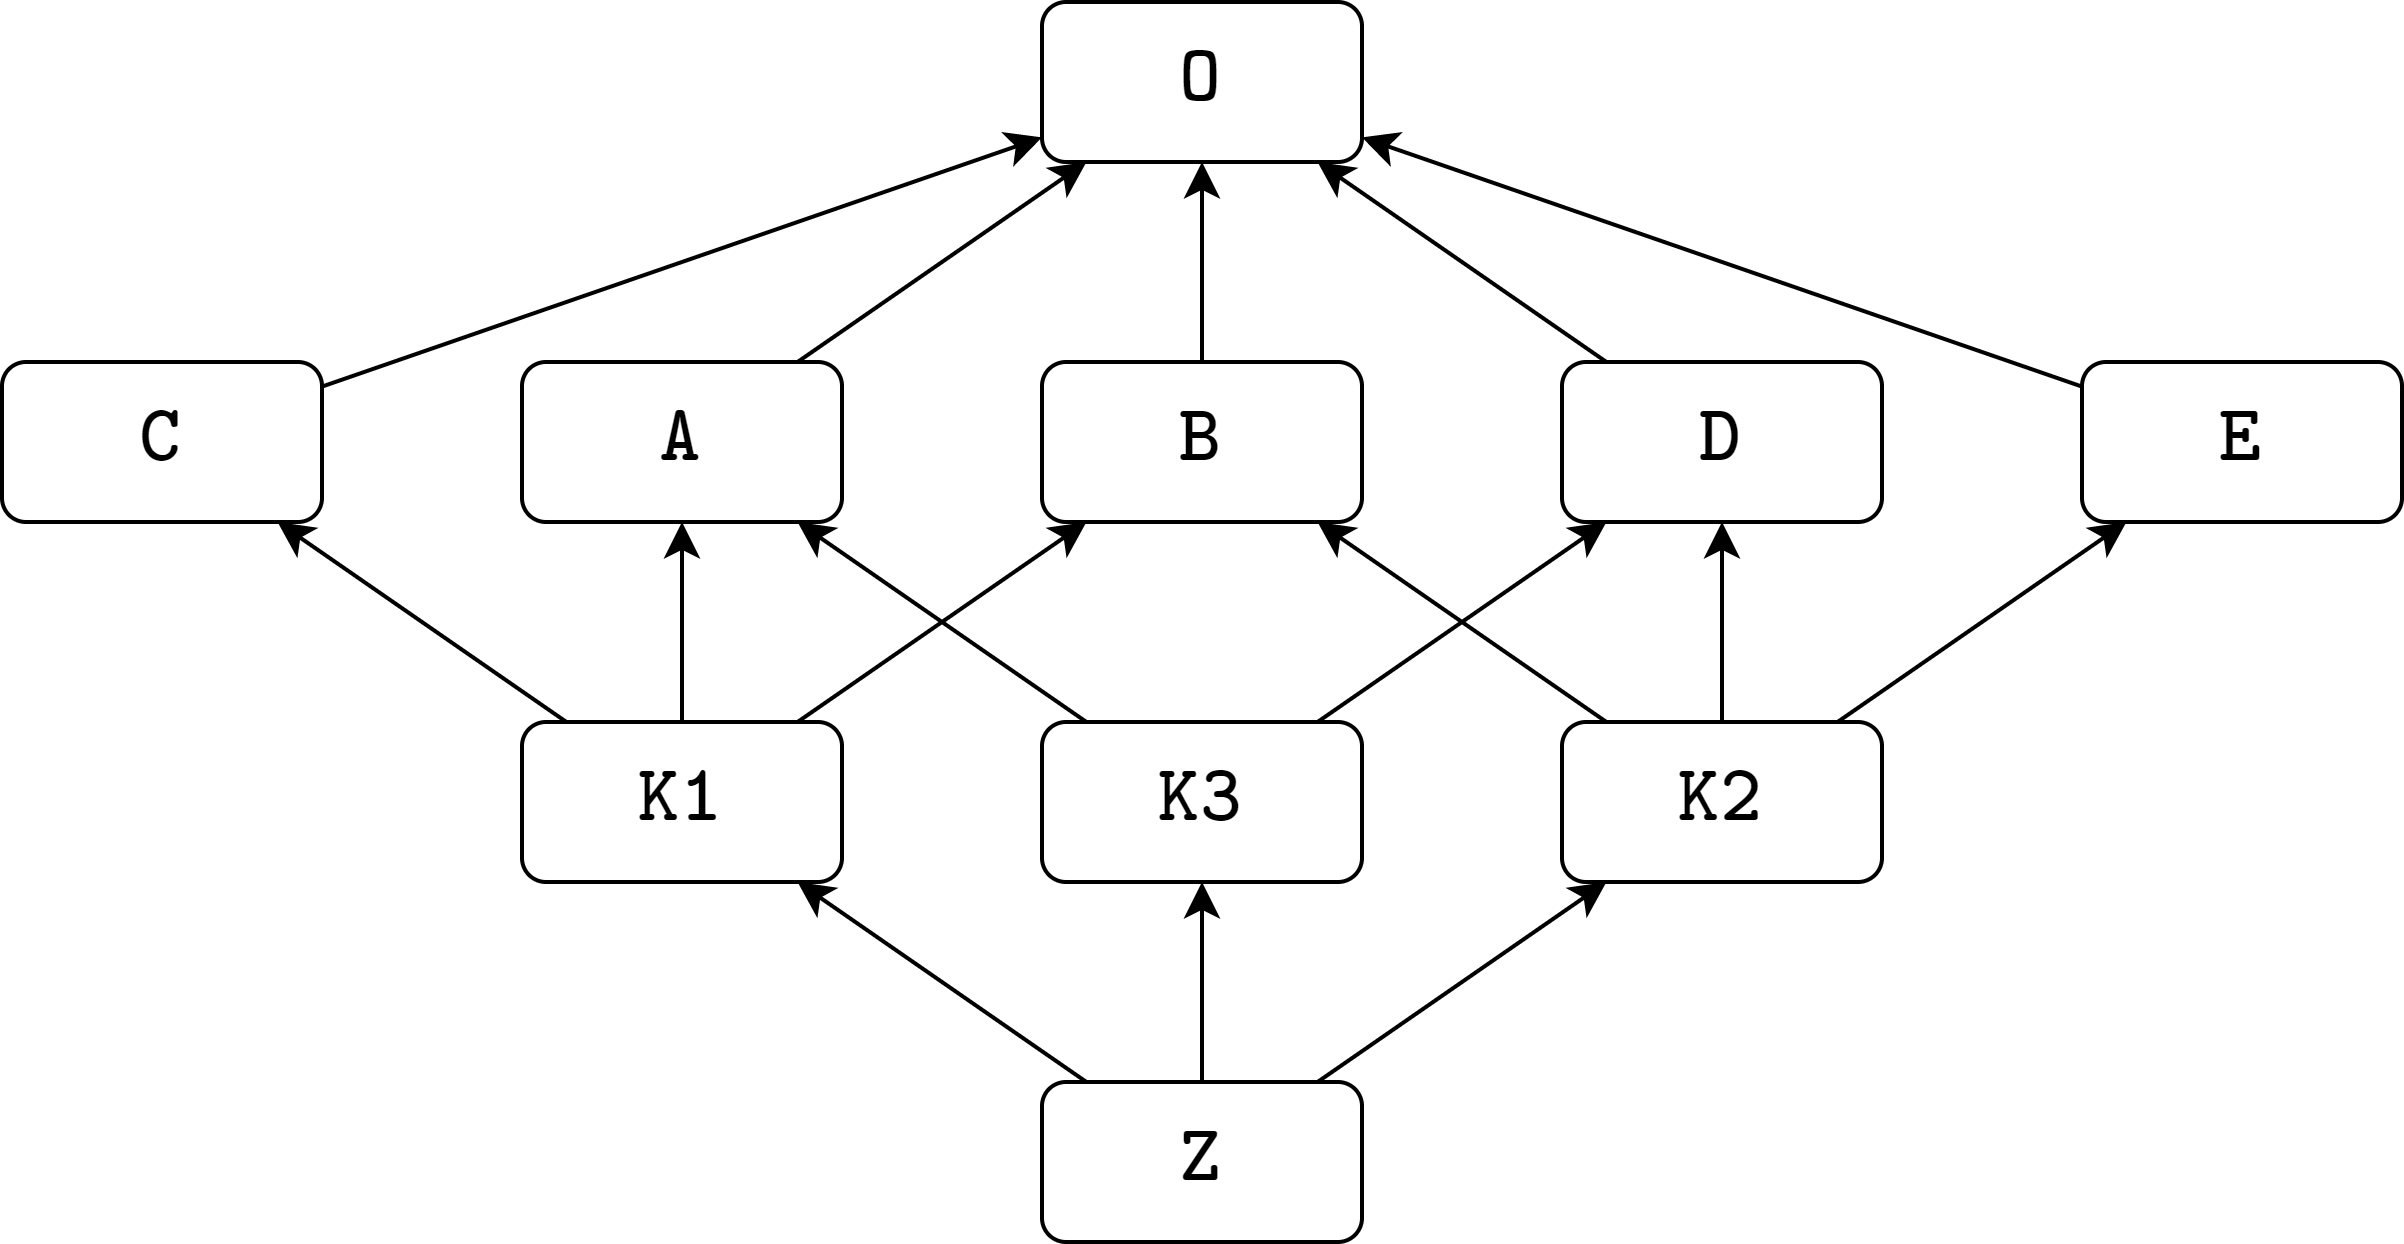
\includegraphics[width=9cm]{./Images/cap3/3.14.png}
    \caption{Linearizzazione C3}
\end{figure}

Un'ABI è un'interfaccia tra due moduli di programma binario, e definisce come si accede alle strutture dati o alle routine nel codice macchina. È espresso in un formato di basso livello, dipendente dall'hardware; al contrario, un'API definisce questo accesso nel codice sorgente, in formato di livello relativamente alto, indipendente dall'hardware.

\subsection{Hyperledger Fabric}
Hyperledger è una famiglia di progetti di blockchain open source avviato a dicembre 2015 dalla Linux Foundation per supportare lo sviluppo collaborativo di soluzioni DLT. Si suddivide in framework per la realizzazione di piattaforme blockchain e strumenti a supporto di applicazioni e smart contracts.

Rispetto ad altre popolari soluzioni ha delle differenze:
\begin{itemize}
    \item ha un'architettura altamente modulare e configurabile;
    \item supporta smart contracts (detto Chaincode) scritti in linguaggi di programmazione comuni, piuttosto che utilizzare linguaggi specifici del dominio;
    \item i partecipanti sono noti, invece che essere anonimi, adottando un modello di governance costruito sulla fiducia che c'è tra i partecipanti;
    \item supporto per protocolli di consenso innestabili, da scegliere sulla base delle esigenze, e senza una criptovaluta nativa per incentivare costosi mining o per alimentare l'esecuzione di contratti intelligenti.
\end{itemize}
Le organizzazioni che prendono parte alla costruzione della rete Hyperledger Fabric sono chiamate \textit{membri}, ognuna responsabile di impostare i propri peer per la partecipazione alla rete. Questi peer devono essere configurati con materiali crittografici appropriati per autenticare la propria identità o proteggere i canali di comunicazione. 

I peer ricevono richieste di transazioni dai client mediante un SDK o servizi web REST per interagire con la rete Hyperledger Fabric, e sono connessi tra loro da canali che consentono l'isolamento dei dati e la riservatezza. Tutti i peer mantengono il loro registro unico per canale a cui sono iscritti, ma a differenza di Ethereum, hanno ruoli diversi:
\begin{itemize}
    \item \textbf{Endorser peer} - ricevuta la richiesta da un client, convalida la transazione ed esegue il Chaincode simulando l'esito della transazione senza aggiornare la blockchain. Al termine, l'Endorser può approvare o disapprovare la transazione. Solo il nodo Endorser esegue il Chaincode, quindi non è necessario installarlo in ogni nodo della rete.
    \item \textbf{Anchor peer} - riceve gli aggiornamenti e trasmette gli aggiornamenti agli altri peer nell'organizzazione. È possibile configurare canali segreti tra i peer, e le transazioni tra i peer di quel canale sono visibili solo ai partecipanti.
    \item \textbf{Orderer peer} - rappresenta l'elemento centrale di un canale tra peer ed è responsabile dello stato del registro coerente in tutta la rete ordinando le transazioni e collocandole in nuovi blocchi. Sono attualmente disponibili due opzioni:
    \begin{itemize}
        \item Solo: un singolo orderer da usare per lo sviluppo, non in produzione, perché poco scalabile e resiliente.
        \item Kafka: soluzione di streaming processing di Apache che garantisce la ricezione di messaggi nell'ordine di invio.
    \end{itemize}
\end{itemize}
Si possono avere due tipi di transazioni: \textit{deploy transactions}, per creare un nuovo chaincode ed installarlo sulla blockchain, ed \textit{invoke transactions}, per richiamare le funzioni di un chaincode. L'applicazione client trasmette la richiesta all'Endorser peer, che controlla i dettagli del certificato e altri dettagli per convalidare la transazione ed eventualmente esegue il chaincode e restituisce le risposte di endorsement, accettando o rifiutando la transazione. Il client invia la transazione approvata all'Ordener peer, affinché questa venga ordinata correttamente rispetto ad altre transazioni ed inclusa in un blocco.

Il nodo Orderer include la transazione di un blocco, e inoltre il blocco ai nodi Anchor di diverse organizzazioni membri della rete, che eseguono un consenso distribuito PBFT.

Al raggiungimento del consenso, gli Anchor peer trasmettono il blocco agli altri peer all'interno della propria organizzazione così che questi aggiornano il proprio registro locale con l'ultimo blocco. Così tutta la rete ottiene il registro sincronizzato.

\vspace{5mm}

Una Certificate Authority (CA) emette i certificati per consentire:
\begin{itemize}
    \item alle organizzazioni di autenticarsi sulla rete;
    \item alle applicazioni client di autenticare le proposte di transazione;
    \item ai peer di approvare le proposte e caricare le transazioni nel libro mastro se valide.
\end{itemize}

Possono esserci una o più CA sulla rete e le organizzazioni possono scegliere di utilizzare una propria CA. La rete viene creata dalla definizione del servizio di ordinazione con la configurazione per i canali all'interno della rete, includendo le politiche di accesso e le informazioni sull'appartenenza (come certificati radice X509) per ogni membro del canale. Il consorzio alla base della rete viene istaurato definendo i certificati delle organizzazioni membro e le relative CA. Un canale C1 è creato generando il blocco di configurazione sul servizio di ordinazione, che valuda la validità della configurazione del canale. L'uso dei canali sono regolati dai criteri con cui sono configurati. I peer vengono uniti ai canali dalle organizzazione che li possiedono e possono esserci più nodi peer sui canali all'interno della rete. P1 è il peer che mantiene copia dello stato della blockchain L1 per le transazioni su C1.

\begin{figure}[htb!]
    \centering
    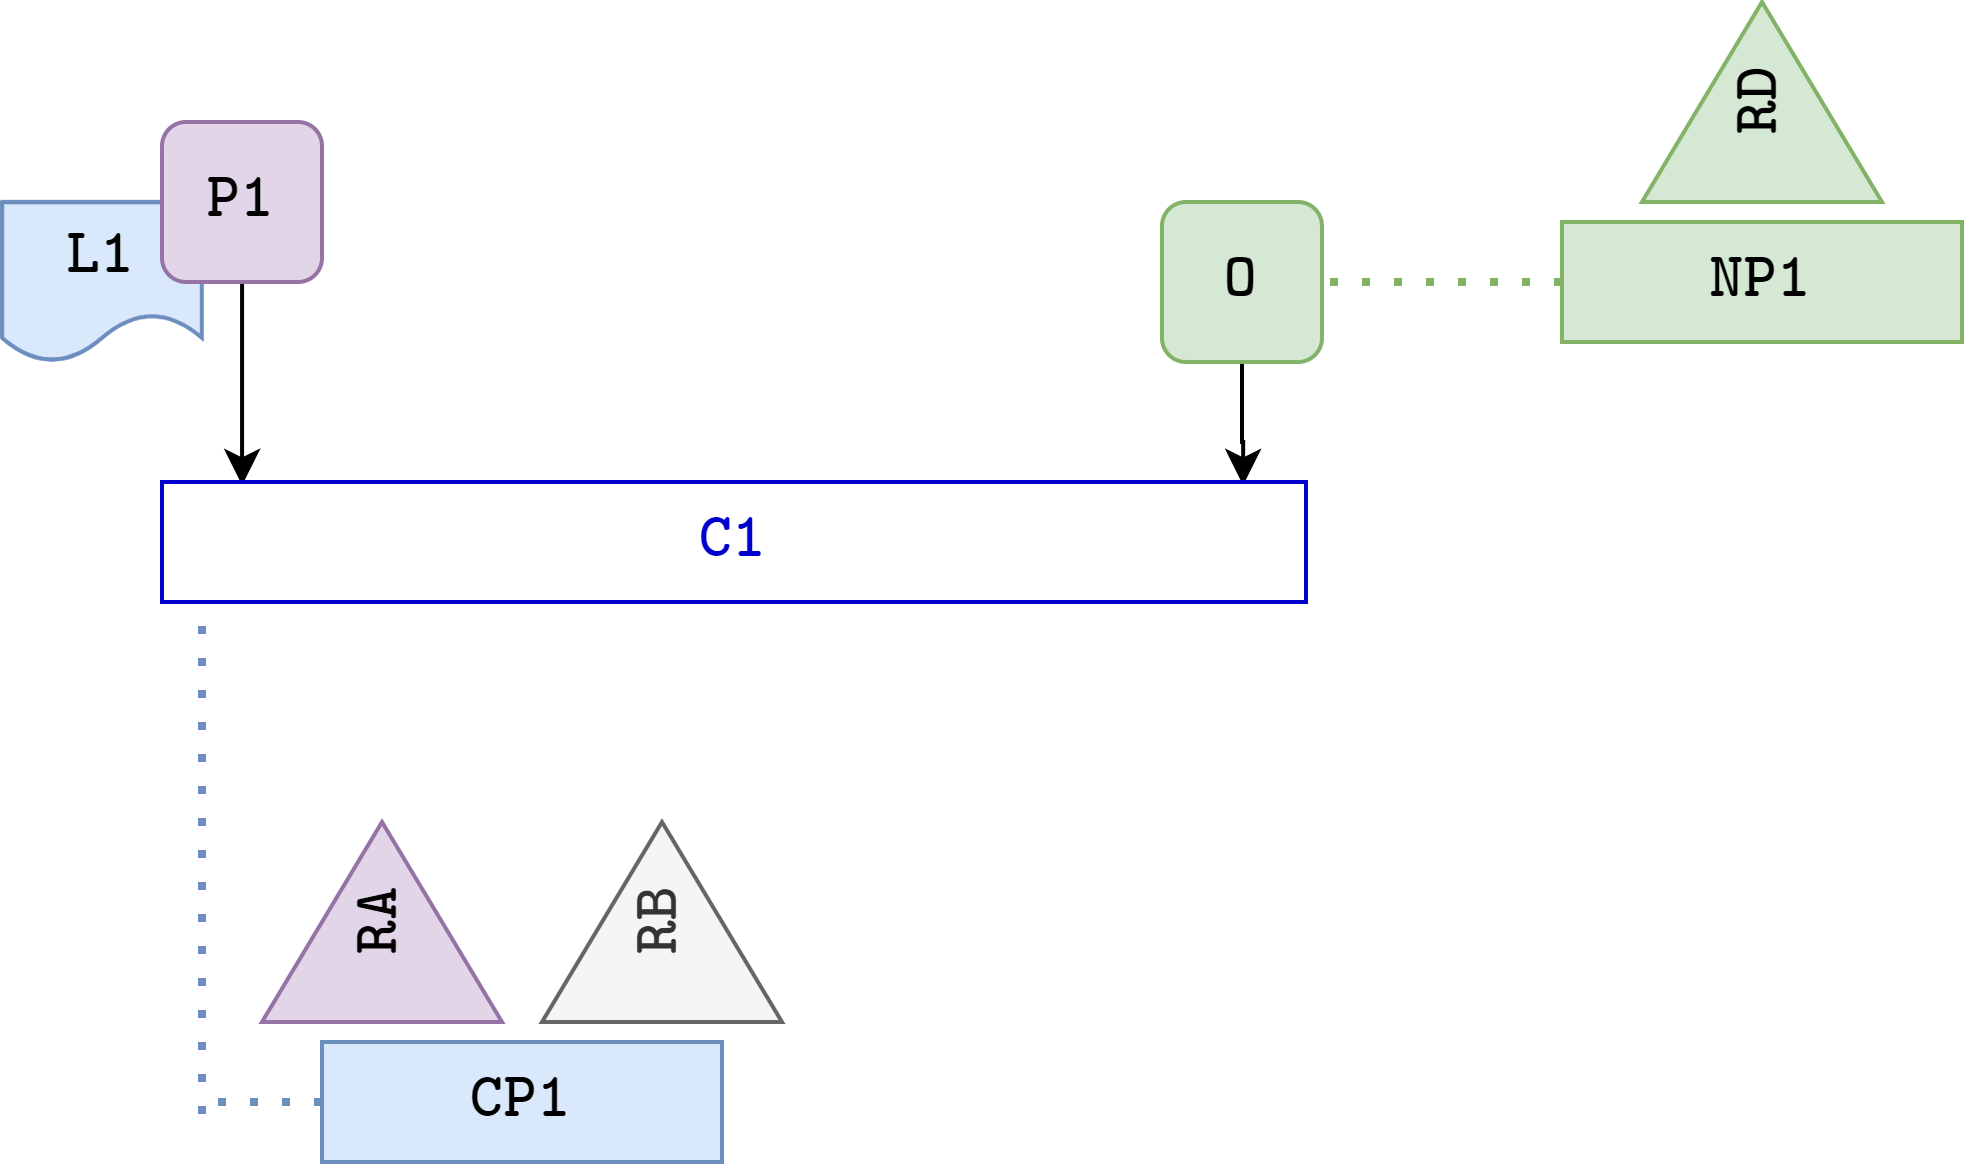
\includegraphics[width=8cm]{./Images/cap3/3.15.png}
\end{figure}

Il libro mastro contiene anche delle informazioni private, accessibili solo ad alcune delle organizzazioni sul canale. Sono contenute in un SideDB e seguono lo stesso processo di endorsement e commit dei dati pubblici, ma la blockchain contiene solo il suo hash. Non ci sono limiti teorici alla dimensione di una rete, e il protocollo gossip è usato per accogliere un gran numero di nodi peer sulla rete.

\vspace{5mm}
 
Nel complesso l'architettura di Hyperledger è composta da tre macro-aree: 
\begin{itemize}
    \item Una per la gestione delle identità, dell'appartenenza di peer ad associazioni e l'iscrizione del peer ai canali.
    \item Un libro mastro con lo stato corrente dei dati e uno storico delle transazioni.
    \item L'ambiente di esecuzione dei chaincode per gli smart contract, diversa da quella di ethereum, che ha un linguaggio di programmazione specifico per gli smart contract (Solidity), infatti in Hyperledger c'`e il concetto di secure container realizzati con un linguaggio di programmazione general purpose.
\end{itemize}
Trasversalmente sono disponibili delle primitive crittografiche a supporto di questi tre strati, che servono per effettuare l'hashing all'interno dei blocchi e per la generazione  e cifratura di token. Questo perché normalmente all'interno dei blocchi non è presente la cifratura del contenuto.

\begin{figure}[htb!]
    \centering
    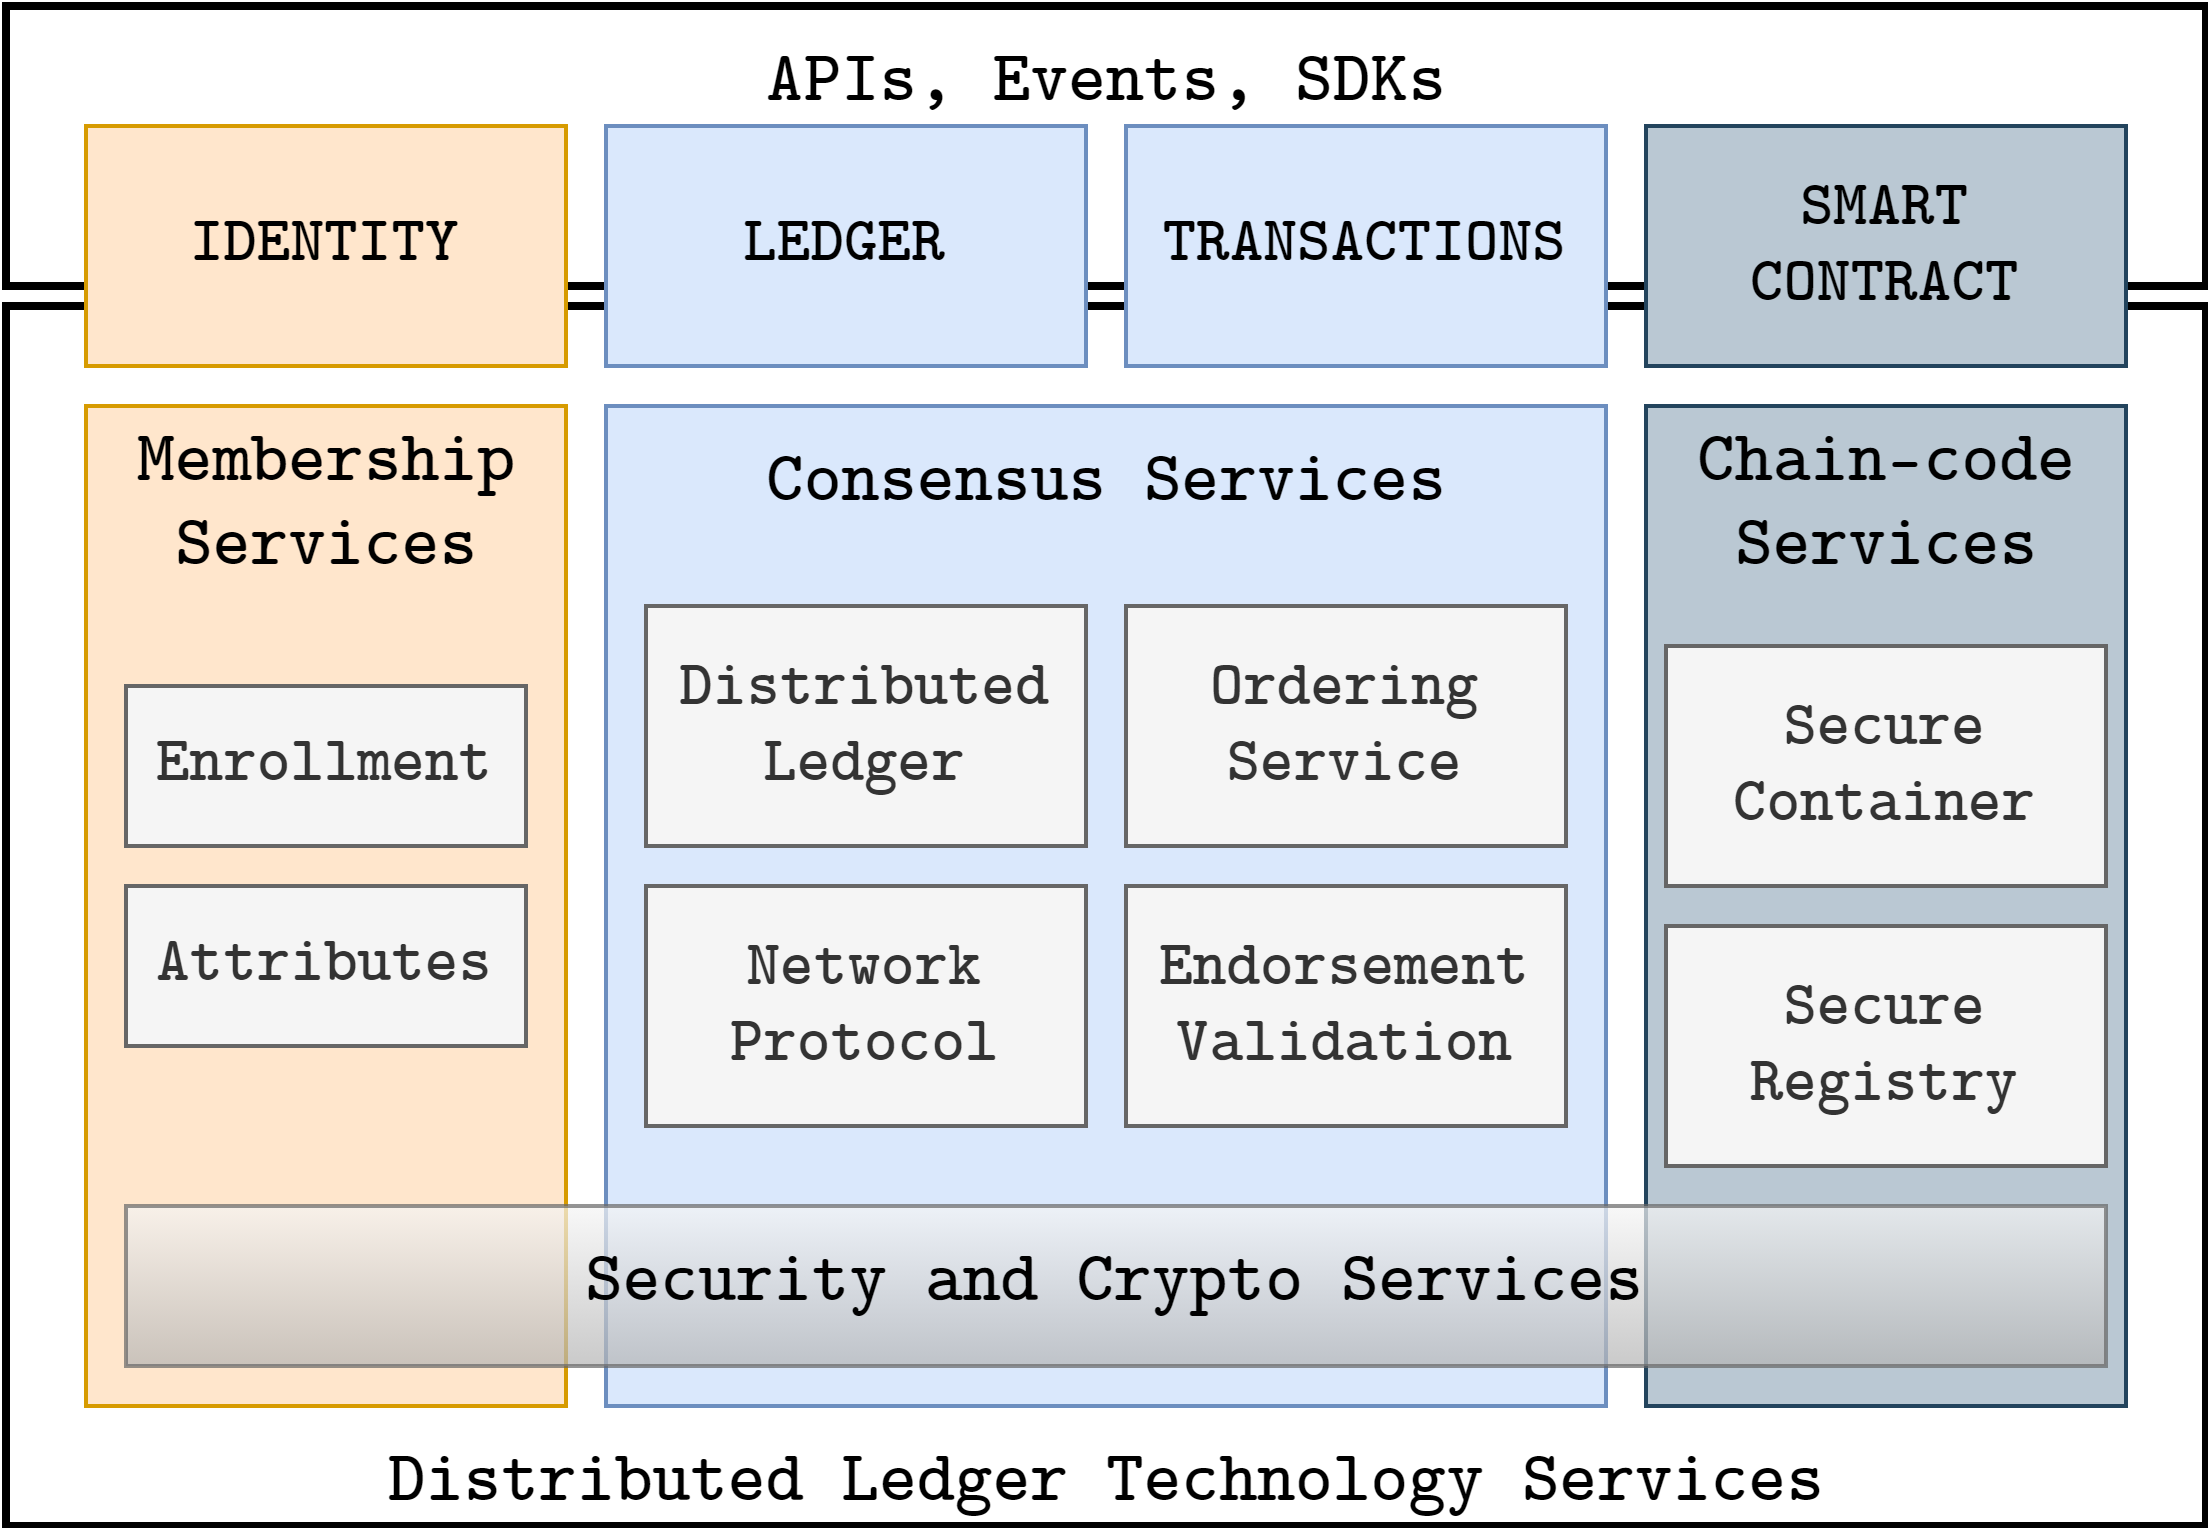
\includegraphics[width=10cm]{./Images/cap3/3.16.png}
\end{figure}

Ogni elemento ha un'identità digitale incapsulata in un certificato digitale X.509, esprimendo anche le autorizzazioni necessarie per le risorse e l'accesso alle funzionalità nella rete blockchain. Affinché un'identità sia verificabile, deve provenire da un'autorità fidata, come la CA con un modello gerarchico PKI. Le Certificate Authority oltre ad avere la possibilità di creare certificati, possiedono anche una lista di certificati revocati, per cui è possibile sempre verificare la validità di un certificato, se questo è rilasciato da una CA.

Il certificato digitale X.509 contiene molte informazioni in merito ad un'identità in SUBJECT, ma anche la chiave pubblica legata all'identità, mentre la sua chiave di firma non lo è e viene mantenuta privata. Il certificato è controfirmato dalla CA che lo emette e lo rende impossibile da modificare, perché viene espresso quale algoritmo è stato utilizzato per la firma imposta dalla CA.

Per motivi di scala esiste una gerarchia di CA, con una Root CA come radice e una serie di CA intermediari i cui certificati sono firmati dalle CA di livello superiore. Fabric offre una propria CA radice firmata da sé stessa, chiamata \textbf{Root of Trust}. Il libro mastro blockchain è costituito da due parti distinte:
\begin{itemize}
    \item un databse che mantiene uno stato globale che contiene i valori correnti di un insieme di dati indirizzabili per mezzo di una chiave (coppia chiave-valore);
    \item collegato allo stato globale abbiamo uno storico delle transazioni come blockchain, con tutti i cambiamenti dello stato globale.
\end{itemize}
Il numero di versione viene incrementato ogni volta che lo stato cambia, e anche verificato ogni volta che lo stato viene aggiornato.

Un blocco ha un header con un numero di sequenza, l'hash del blocco e del blocco precedente, il corpo con l'insieme ordinato delle transazioni e dei metadati con l'ora di creazione del blocco, il certificato, la chiave pubblica e la firma del creatore del blocco. Le transazioni hanno un header come il nome del chaincode pertinente e la sua versione, la firma del creatore, la proposta e la risposta con l'endorsement. Da ricordare che Hyperledger non ha un sistema di criptovalute come Ethereum, per cui le transazioni rappresentano invocazioni di chaincode.

\subsubsection{\textbf{CHAINCODE}}

\textbf{Chaincode} è uno smart contract nell'ambiente Hyperledger Fabric ed è un programma scritto in Go, Node.js o Java che implementa un'apposita interfaccia e viene eseguito in un contenitore Docker per garantire al peer che sta eseguendo l'endorsement di eseguire la verifica in un ambiente isolato. Lo stato creato da un chaincode è limitato esclusivamente a quel chaincode e non è possibile accedervi direttamente da un altro chaincode. Tuttavia, un chaincode può invocare un altro chaincode per accedere al suo stato.

L'interfaccia Chaincode specifica le funzioni da implementare (circa 36), di cui le due più importanti sono:
\begin{itemize}
    \item \texttt{init()} viene chiamato quando un chaincode viene deployato per la prima volta o riceve un'istanza o una transazione di aggiornamento in modo da eseguire qualsiasi inizializzazione necessaria, inclusa quella dello stato dell'applicazione;
    \item \texttt{invoke()} viene chiamato in risposta alla ricezione di una transazione per elaborare le proposte di transazione assegnate al chaincode.
\end{itemize}
L'altra interfaccia è \texttt{ChaincodeStubInterface}, che viene utilizzata per accedere e modificare la blockchain e per effettuare invocazioni tra in chaincode. Dato che il supporto Java è stato introdotto di recente, le API Node.js e Go sono a un livello più maturo. JavaScript invece non si presta bene nel caso di calcoli numerici. Il linguaggio più usato per la realizzazione di chaincode è Go: questo non presenta il concetto di classe ma offre struct, una versione leggera delle classi a cui è possibile aggiungere metodi. La differenza tra struct e classi è che nelle struct i membri sono tutti pubblici per default, mentre nelle classi esiste il concetto di incapsulamento e membri privati. Inoltre nelle struct di Go lang non è possibile definire i metodi. Nella sintassi di Go lang dopo la parola chiave \texttt{func} sono indicati i tipi di oggetti che possono chiamare quella funzione.

Vediamo un esempio di realizzazione di smart contract in Go per la gestione delle auto e dei loro proprietari:

\begin{lstlisting}[language=Go]

type Car struct{
  modelName string
  color string
  serialNo string
  manufacturer string
  owner Owner  //composition
}

type Owner struct{
  name string
  nationalIdentity string
  gender string
  address string
}

//attached by reference -> called as pointer receiver
func (c *Car) changeOwner(newOwner Owner){
  c.owner = newOwner
}

//attached by value -> called as value receiver
func (c Car) changeOwner(newOwner Owner){
  c.owner = newOwner
}

/*queste due funzioni possono essere chiamate da oggetti Car, nel primo caso da riferimenti a tipo Car, mentre nel secondo caso da oggetti di tipo Car. Nel primo caso le modifiche nel corpo del metodo si riflettono sul chiamante, mentre nel secondo caso viene effettuata una copia.*/

\end{lstlisting}

\subsubsection{COSTRUZIONE DI UNO SMART CONTRACT}

L'interfaccia da implementare è la seguente con le due principali funzioni delle 36 attualmente specificate:

\begin{lstlisting}[language=Go]

type Chaincode interface {
//Init method accepts stub of type ChaincodeStubInterface as
//argument and returns peer.Response type object
  Init(stub ChaincodeStubInterface) peer.Response
  Invoke(stub ChaincodeStubInterface) peer.Response
}

\end{lstlisting}
Non sussiste una sintassi di derivazione, ma basta solo implementare i metodi di interesse. Il tipo di ritorno è indicato alla fine e non all'inizio.
\begin{lstlisting}[language=Go]

type CarChaincode struct{
}

//Init implemented by CarChaincode
func (t *CarChaincode) Init(stub shim.ChaincodeStubInterface)
  pb.Response {
  
}

//Invoke implemented by CarChaincode
func (t *CarChaincode) Invoke(stub shim.ChaincodeStubInterface)
  pb.Response {
  
}

//pb e shim sono le librerie importate

\end{lstlisting}

\subsubsection{\textbf{Costruzione di uno smart contract}}

Inseriamo la logica di inizializzazione: la funzione \texttt{Init()} carica uno stato iniziale sulla blockchain. Dopodiché  salvo le struct in variabili di tipo json. La funzione GetState fa una query sul DB di hyperledger fabric per controllare lo stato.
\begin{lstlisting}[language=Go]

func (t *CarChaincode) Init(stub shim.ChaincodeStubInterface)
  pb.Response {
  
  //Declare owners from Owner struct
  tom := Owner{name: "Tom H", nationalIdentity: "ABCD33457", gender:
  "M", address: "1, Tumbbad"}
  bob := Owner{name: "Bob M", nationalIdentity: "QWER33457", gender:
  "M", address: "2, Tumbbad"}
  
  //Declare car from Car struct
  car := Car{modelName: "Land Rover", color: "white", serialNo:
  "334712531234", manufacturer: "Tata Motors", owner: tom}
  
  //Convert tom Owner to []byte
  tomAsJSONBytes, _ := json.Marshal(tom)
  //Add Tom to ledger
  err := stub.PutState(tom.nationalIdentity, tomAsJSONBytes)
  if err != nil {
    return shim.Error("Failed to create asset " + tom.name)
  }
  
  //Add Bob to ledger
  bobAsJSONBytes, _ := json.Marshal(bob)
  //Add Tom to ledger
  err := stub.PutState(bob.nationalIdentity, bobAsJSONBytes)
  if err != nil {
    return shim.Error("Failed to create asset " + bob.name)
  }
  
  //Add car to ledger
  carAsJSONBytes, _ := json.Marshal(car)
  //Add Tom to ledger
  err := stub.PutState(car.serialNo, carAsJSONBytes)
  if err != nil {
    return shim.Error("Failed to create asset " + car.serialNo)
  }
  
  return shim.Success([]byte("Assets created successfully."))
}

\end{lstlisting}

Inseriamo la logica di Invoke:

\begin{lstlisting}[language=Go]

func (c *carChaincode) Invoke(stub shim.ChaincodeStubInterface)
 pb.Response{
 
 //Read args from the transaction proposal
 //fc -> method to invoke
 fc, args := stub.GetFunctionAndParameters()
 if fc == "TransferOwnership" {
   return c.TransferOwnership(stub, args)
 }
 return shim.Error("Called function isn't defined in the chaincode")
}

func (c *CarChaincode) TransferOwnership(stub
  shim.ChaincodeStubInterface, args []string) pb Response {
  //args[0] -> car serial no
  //args[1] -> new owner national identity
  //Read existing car asset
  carAsBytes, _ := stub.GetState(args[0])
  if carAsBytes == nil {
    return shim.Error("car asset not found")
  }
  
  //Construct the struct Car
  car := Car{}
  _ = json.Unmarshal(carAsBytes, &car)
  
  //Read newOwner details
  ownerAsBytes, _ := stub.GetState(args[1])
  if ownerAsBytes == nil {
    return shim.Error("owner asset not found")
  }
  
  //Construct the struct Owner
  newOwner := Owner{}
  _ = json.Unmarshal(ownerAsBytes, &mewOwner)
  
  //Update owner
  car.changeOwner(newOwner)
  
  carAsJSONBytes, _ := json.Marshal(car)
  
  //Update car ownership
  err := stub.PutState(car.serialNo, carAsJSONBytes)
  if err != nil {
    return shim.Error("Failed to create asset " + car.serialNo)
  }
  
  return shim.Success([]byte("Assets modified."))
}

\end{lstlisting}

Per completare lo smart contract è necessario specificare il preambolo:

\begin{lstlisting}[language=Go]

package main

import (
  "encoding/json"
  
  "github.com/hyperledger/fabric/core/chaincode/shim"
  pb "github.com/hyperledger/fabric/protos/peer"
  )

\end{lstlisting}

E la funzione principale:
\begin{lstlisting}[language=Go]

func main() {
  logger.SetLevel(shim.LogInfo)
  
  //Start chaincode process
  err := shim.Start(new(CarChaincode))
  if err != nil {
    logger.Error("Error starting PhantomChaincode - ", err.Error()
  }
}

\end{lstlisting}
